%% LyX 2.0.4 created this file.  For more info, see http://www.lyx.org/.
%% Do not edit unless you really know what you are doing.
\documentclass[10pt,twocolumn,letterpaper]{article}
\usepackage{cvpr}
\usepackage[T1]{fontenc}
\usepackage[latin9]{inputenc}
\usepackage{geometry}
\geometry{verbose, margin = 1in}
\usepackage{amsthm}
\usepackage{amsmath}
\usepackage{tikz}
\usepackage{array}
\usetikzlibrary{arrows}

\setlength{\parskip}{0.63pc}


\makeatletter
%%%%%%%%%%%%%%%%%%%%%%%%%%%%%% Textclass specific LaTeX commands.
\numberwithin{equation}{section}
\numberwithin{figure}{section}
\theoremstyle{plain}
\newtheorem{thm}{\protect\theoremname}
  \theoremstyle{definition}
  \newtheorem{defn}[thm]{\protect\definitionname}
  \theoremstyle{plain}
  \newtheorem{lem}[thm]{\protect\lemmaname}

\makeatother

\usepackage{babel}
  \providecommand{\definitionname}{Definition}
  \providecommand{\lemmaname}{Lemma}
\providecommand{\theoremname}{Theorem}

% Useful macro commands.
\newcommand*{\bigtheta}[1]{\Theta\left( #1 \right)}
\newcommand*{\bigo}[1]{O \left( #1 \right)}
\newcommand*{\bigomega}[1]{\Omega \left( #1 \right)}
\newcommand*{\prob}[1]{\text{Pr} \left[ #1 \right]}
\newcommand*{\ex}[1]{\text{E} \left[ #1 \right]}
\newcommand*{\var}[1]{\text{Var} \left[ #1 \right]}

\newcommand*{\norm}[1]{\left\lVert #1 \right\rVert}
\newcommand*{\HH}{\mathscr{H}}   % Family of hash functions.
\newcommand*{\UU}{\mathscr{U}}   % Universe.
\newcommand*{\eps}{\varepsilon}  % Epsilon.


\cvprfinalcopy

\ifcvprfinal\pagestyle{empty}\fi
\begin{document}

\title{Analyzing Hollow Heap Varients and their Computational Properties}


\author{
  Luis Perez \\
  Department of Computer Science \\
  Stanford University \\
  \texttt{luis0@stanford.edu}
  
  \and
  Dana Murphy  \\
  Department of Computer Science\\
  Stanford University\\
  \texttt{dkm0713@stanford.edu}
  
  \and
  
  \\
  Eric Martin \\
  Department of Computer Science \\
  Stanford University \\
  \texttt{ericmarkmartin@stanford.edu}
}

\maketitle

\section{Introduction}
\label{sec:introduction}
In this paper, we motivate, introduce, describe, and expand on existing work surrounding the relatively novel data structure (2015) of Hollow Heaps, as first described by Hansen, Kaplan, Tarjan, and Zwich \cite{HollowHeapsIntro}. A Hollow Heap is primarily a data structure designed to provide an efficient and simple mechanism for extracting the element with the minimum key in a set of $n$ elements, subject to the constraints that insertions, deletions, and key changes can occur dynamically and must also be supported efficiently. One-root, single-parent Hollow Heaps are one of the more simple data structures to achieve $O(\log n)$ amortized run-time for min-extraction, along with $O(1)$ run-time for all other operations. This paper presents a detailed analysis of the original data structure as well as expanded and detailed analaysis of multiple varients which provide distinct trade-offs.


\section{Problem and Objective}
\label{sec:problem_and_objective}
The problem consists of defining a data structure $Q$, called a Priority Queue, that can support the following five operations in an efficient manner:

\begin{itemize}
    \item \texttt{Meld}$(h_1, h_2) \rightarrow h_3$: Returns a new heap $h_3$ containing all items from heaps $h_1$ and $h_2$.
    \item \texttt{Insert}$(Q,x,k) \rightarrow \bar{x}$ - insert an item $x$ with key $k$ into heap $Q$ and return a reference $\bar{x}$ to $x$.
    \item \texttt{ExtractMin}$(Q) \rightarrow k $ - remove the minimum item from the heap $Q$ and return the key $k$ associated with it
    \item \texttt{DecreaseKey}$(Q, \bar{x}, k') \rightarrow \texttt{None}$  - given a handle $\bar{x}$, change the key of item $x$ contained in the heap $Q$ to be $k'$. It is guaranteed that $k' \leq k$, the original key.
    \item \texttt{FindMin}$(Q) \rightarrow x$ - finds and returns the element with the minimum key in $Q$. $Q$ is left unmodified.
\end{itemize}

One concrete data structure that is often used to support priority queue operations is called a heap. Conceptually, a heap is simply a tree in which every node $n$ with parent node $m$ have keys $n_k$ and $m_k$ respectively such that $n_k > m_k$ (this is called a min-heap---in a max-heap, $n_k < m_k$). Many variants of heaps exist, supporting the above operations. A few popular ones include the Binary Heap, Leftist Heap, Binomial Heap, Fibonacci Heap, and the Pairing Heap. We have provided a summary of their run-times in Table \ref{table:heap_complexity_reference} for reference. 

Fibonacci Heaps \cite{FibHeapsRevisited} are a particularly well-known, theoretically efficient implementation of a priority queue. As we can see in Table \ref{table:heap_complexity_reference}, Fibonacci heaps offer amortized $O(\log n)$ for \texttt{ExtractMin} along with amortized $O(1)$ run-time for other operations. While these remarkable amortized bounds have helped popularize this algorithm, it remains a conceptually difficult data structure, requiring a rather in-depth understanding of amortized analysis and binomial heaps. While alternative data structures to Fibonacci heaps have been proposed, many of them don't match the bounds of Fibonacci Heaps (e.g. Quake heaps), focus on simplifying Fibonacci heap in small ways (e.g. Strict Fibonacci Heap), or provide an algorithm that is as complex or more complex than Fibonacci heaps (e.g. Worst-Case priority queues)\cite{waybackMachine}.

\begin{table*}[!ht]
\centering
\begin{tabular}{l|l|l|l|l|l|}
\cline{2-6}
& \textbf{Binary} & \textbf{Leftist} & \textbf{Binomial} & \textbf{Fibonacci} & \textbf{Pairing} \\ \hline
\multicolumn{1}{|l|}{\textbf{Meld}}        & O(n)            & O(log n)         & O(log n)          & O(1)               & O(1)             \\ \hline
\multicolumn{1}{|l|}{\textbf{Insert}}      & O(log n)        & O(log n)         & O(1)              & O(1)               & O(1)             \\ \hline
\multicolumn{1}{|l|}{\textbf{ExtractMin}}   & O(log n)        & O(log n)         & O(log n)          & O(log n)           & O(log n)         \\ \hline
\multicolumn{1}{|l|}{\textbf{DecreaseKey}} & O(log n)        & O(log n)         & O(log n)          & O(1)               & O(1)             \\ \hline
\multicolumn{1}{|l|}{\textbf{FindMin}}     & O(1)            & O(1)             & O(log n)          & O(1)               & O(1)             \\ \hline
\end{tabular}
\caption{A matrix showing typical run-times of some variant implementation of the abstract heap data structure. Of interest is the theoretical advantage of Fibonacci Heaps across the board, with all but one operation running in constant time.}
\label{table:heap_complexity_reference}
\end{table*}

Our primary objective in this paper is to introduce and analyze the most salient properties of Hollow Heaps \cite{HollowHeapsIntro}, a variant of the Heap implementation above that can ultimately be made to achieve the same run-times as Fibonacci Heaps (See Table \ref{table:heap_complexity_reference}), but has a more simple design than Fibonacci Heaps and other equally-efficient alternatives like Pairing Heap. 

Mainly, we provide a new insight into Hollow Heaps by showing that the simplest variant of Hollow Heaps is essentially a lazier Fibonacci Heap, where the work which normally occurs during a \texttt{DecreaseKey} operation in Fibonacci Heaps is moved to the \texttt{ExtractMin} operation. With this insight we can draw from our knowledge of equivalent Fibonacci Heap properties to explore different aspects of Hollow Heaps and its many variants.

Lastly, we explore the idea of keeping the number of hollow nodes in hollow heaps manageable. To do this, we explore the concept of hollow leaf removal, analyzing how this would influence the amortized runtime and how this could mitigate the ratio of hollow to full nodes. Next, we explore the concept of \textit{reviving} Hollow Nodes, or filling nodes that were previously made hollow as well, and the applications where Hollow Heaps with Revival would be particularly useful.


\section{A Lazier Fibonacci Heap}
\label{sec:lazier_f-heap}

Conceptually Hollow Heaps \cite{waybackMachine} share much of their design with Fibonacci Heaps. Both algorithms are built on top of binomial heaps, rely on lazy insertions and melds with most of the work being done in extract-min, and maintain a bound on the minimum number of nodes that can be descendants of a node with a given rank. However, the primary difference between Fibonacci Heaps and the most basic implementation of Hollow Heaps is how they handle decrease keys and deletions. Namely, Fibonacci heaps use a somewhat lazy algorithm for deleting and decreasing keys, while Hollow Heaps use an even lazier method for handling deletes and key decreases.

%%%%%%%%% BEGIN: SECTION COVERING FibHeaps %%%%
\subsection{A refresher on DecreaseKey \& Delete in Fibonacci Heaps}
\label{subsec:decrease_key_refresher}

Fibonacci Heaps rely on two keys ideas to achieve amortized $O(1)$ run-time for \texttt{DecreaseKey}.

\begin{itemize}
    \item Cut nodes from the tree (and create a new root in the process) if they violate the heap invariant after their key decreases (see Figure \ref{fig:fibHeapDecreaseKey} for an example)
    \item If ever a node loses two children, also cut that node from the tree (see Figure \ref{fig:fibHeapDecreaseKey} for an example)
\end{itemize}

As a reminder, Fibonacci heaps maintain an invariant that a node of rank $r$ has at least $F_{r+3} - 1$ descendants, and the invariant that the rank of any given node is at most $log_{\phi} n$.
    
\begin{figure}
    \centering
    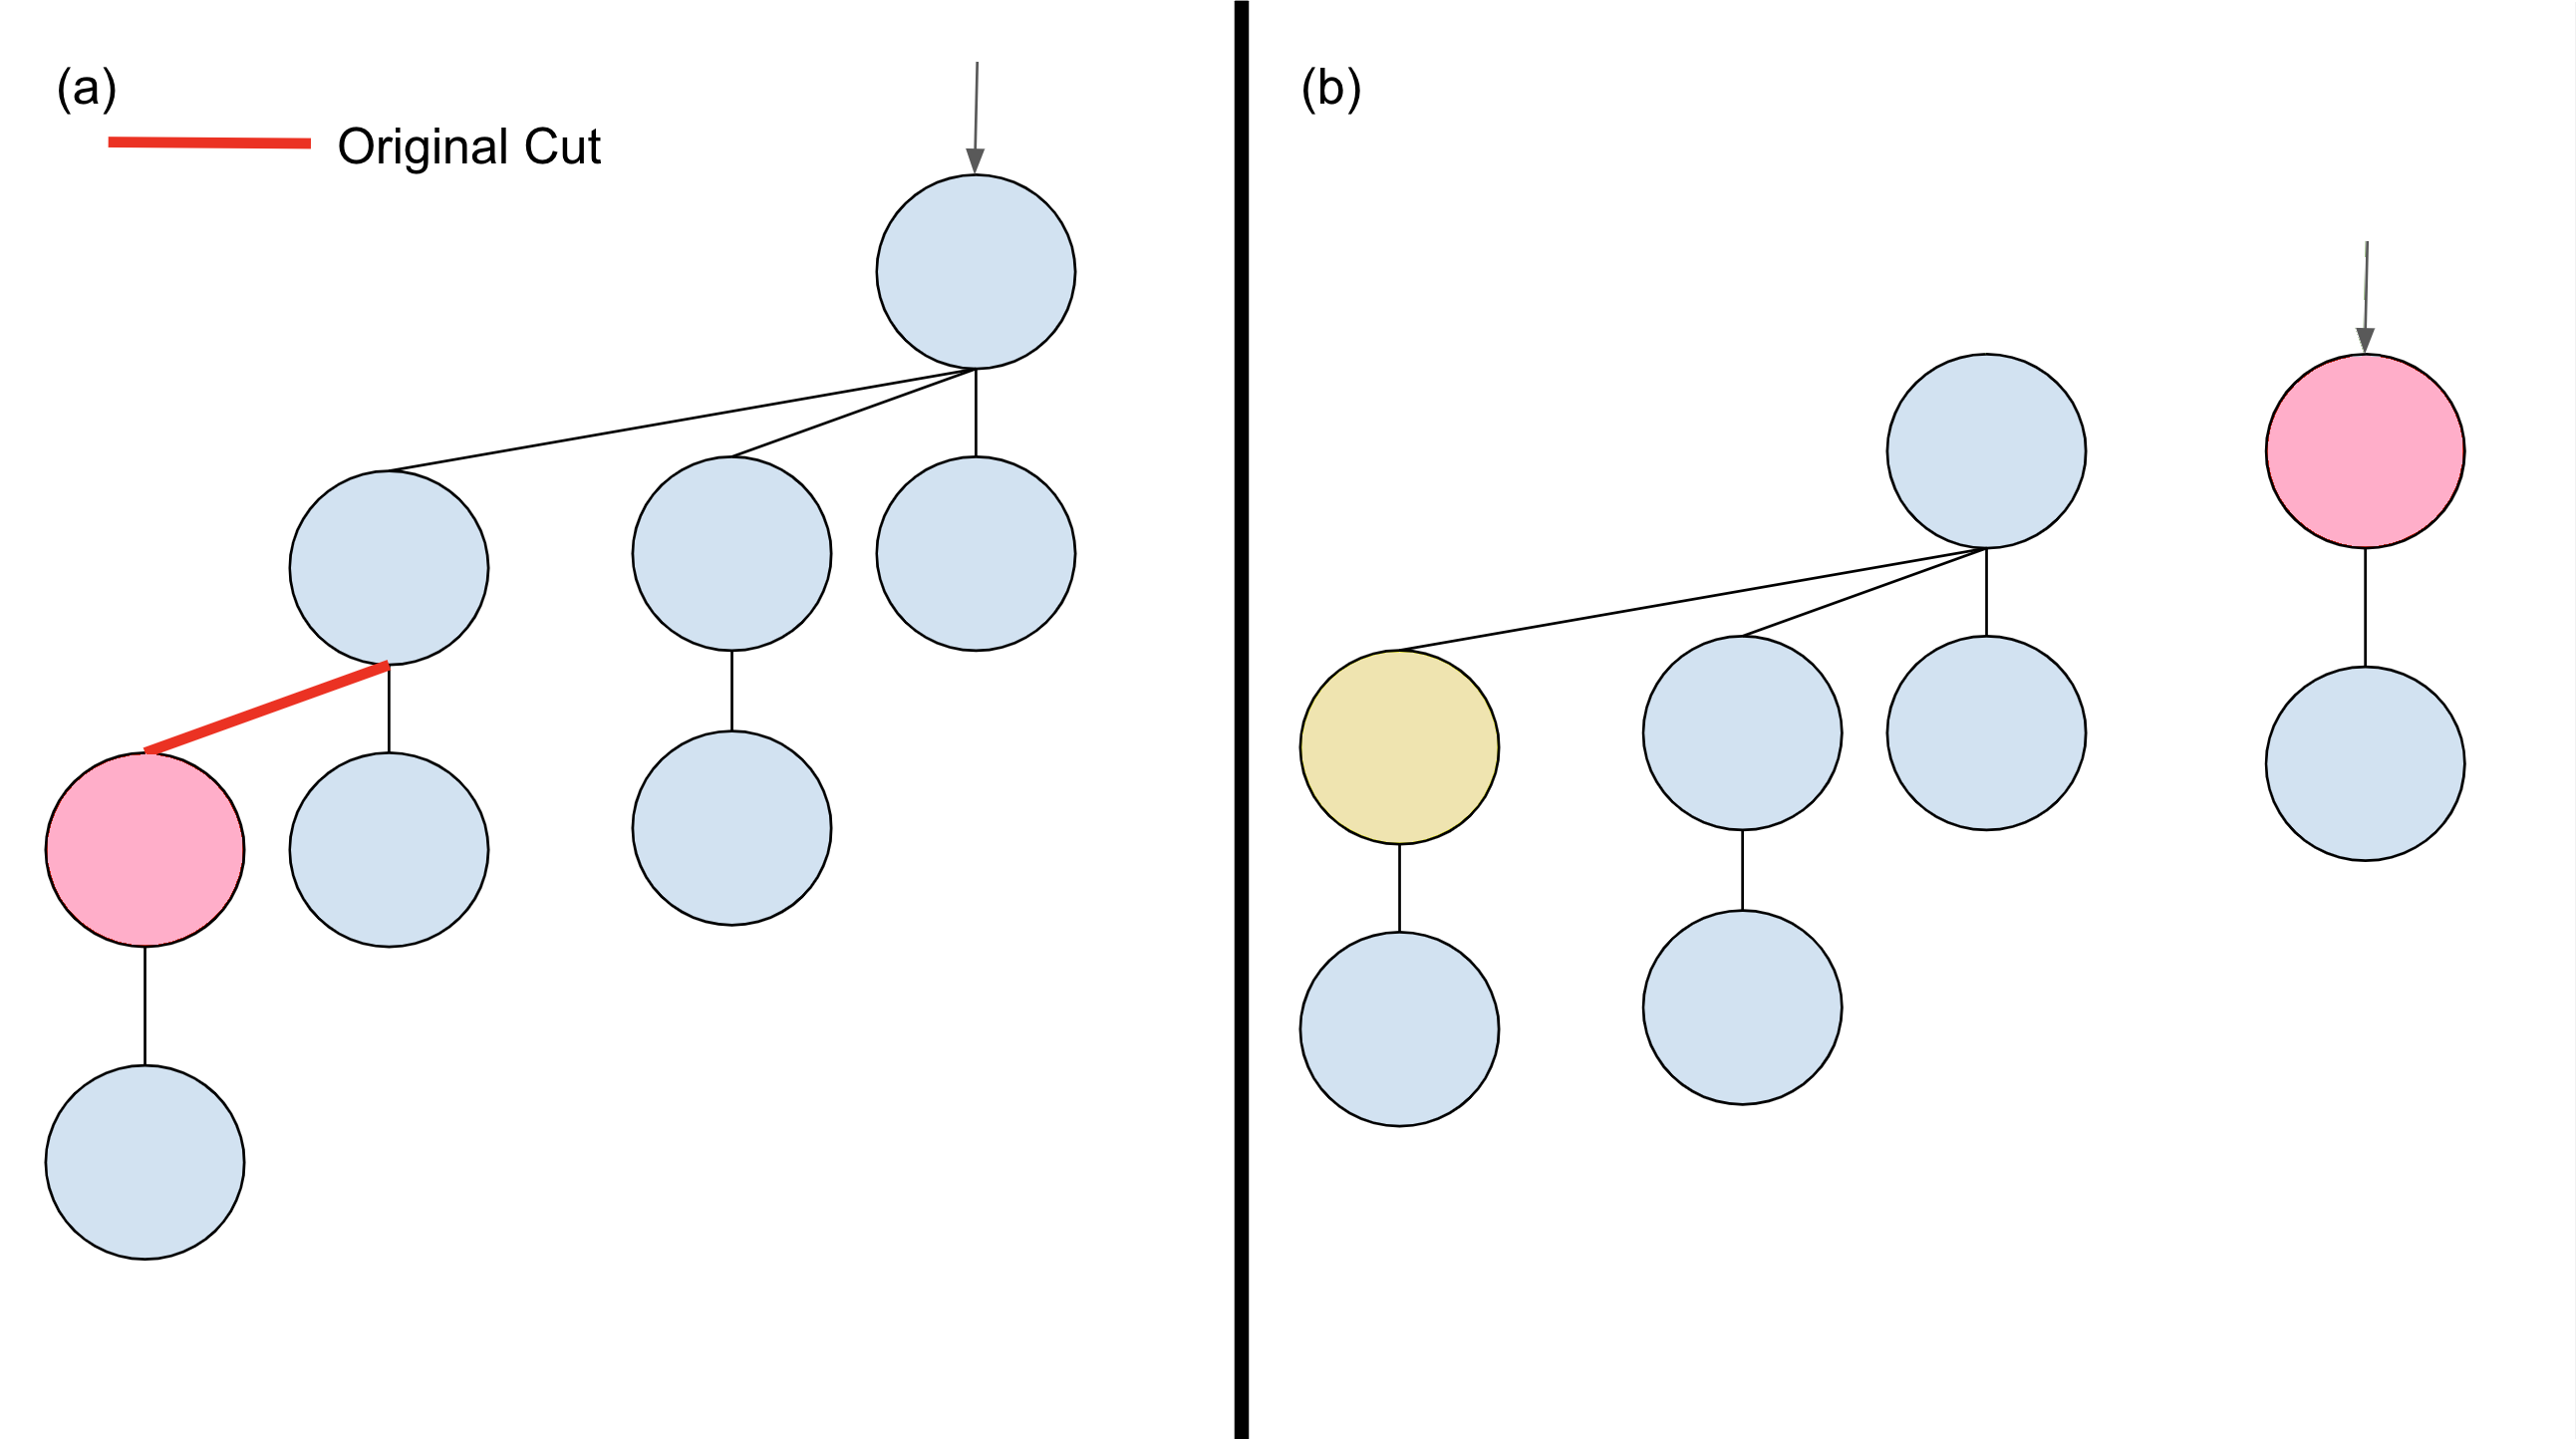
\includegraphics[scale=0.10]{figures/FibonacciHeap-DecreaseKey-1Cut-new.png}
    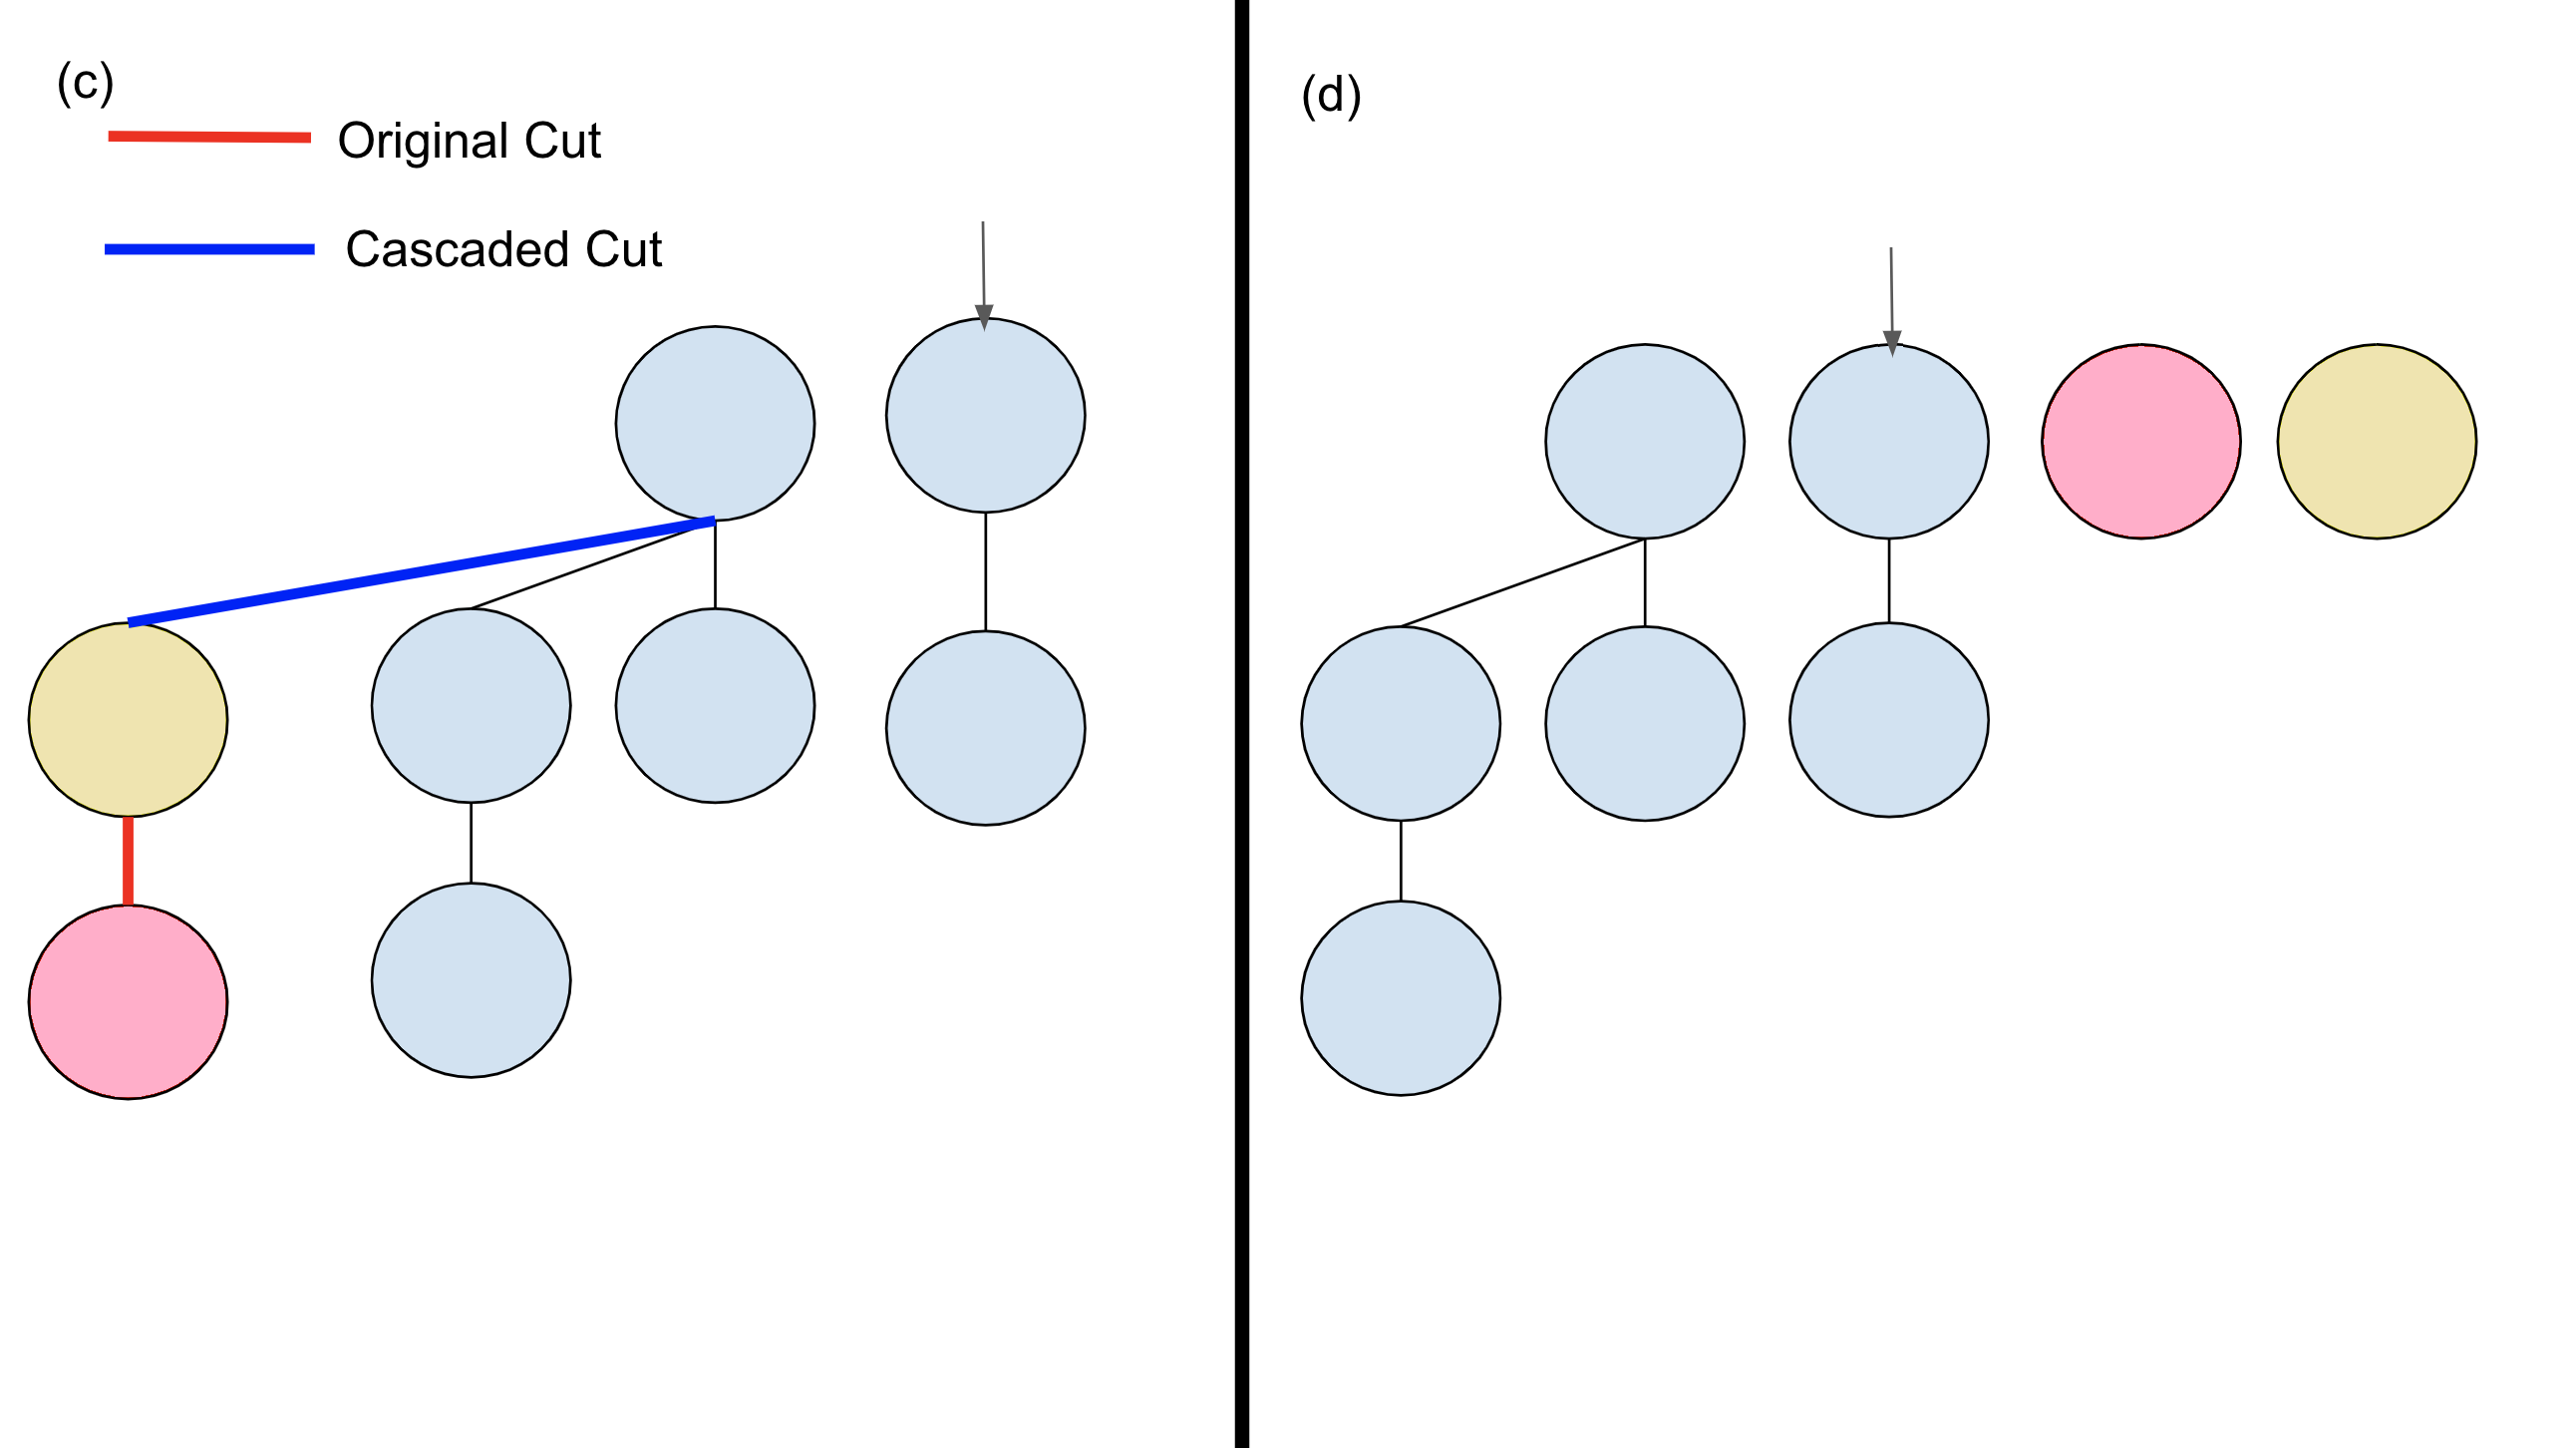
\includegraphics[scale=0.10]{figures/FibonacciHeap-DecreaseKey-2Cut-new.png}
    \caption{An example of the work performed in a Fibonacci Heap during \texttt{DecreaseKey} operations. From (a) to (b), we're decreasing the key of the pink node, which removes that subtree from the tree and marks the parent (yellow). From (c) to (d), we're again removing a node (pink), but this time the parent (yellow) has now lost two children, and so much be removed too. These are the \textit{cascading} cuts in Fibonacci Heap.}
    \label{fig:fibHeapDecreaseKey}
\end{figure}


%%\begin{thm}
%%A single \texttt{DecreaseKey} operation in a traditional Fibonacci Heap can trigger up to $\Theta(\log n))$ operations.
%%\end{thm}

%%TODO: potential cut if paper is getting too long.
%%\begin{proof}
%%The proof is rather straight-forward. Just consider a Fibonacci Heap with a single tree where all nodes along a path have had at least one-child removed (due to previous \texttt{DecreaseKey} operations. Then a \texttt{DecreaseKey} operation on the deepest node along this path will cause $\Theta(\log n)$ cascading cuts.
%%\end{proof}

%%The above description of Fibonacci Heaps is sufficient to introduce some motivation for Hollow Heaps.

%%%%%%%%% END: SECTION COVERING FibHeaps %%%%

%%%%%%%%% START: SECTION COVERING HollowHeapMotivate %%%%
\subsection{What are Hollow Nodes?}
\label{subsec:hollow_nodes}
Hollow Heaps provides an alternative to the cascading cuts that occur in Fibonacci heaps, while still maintaining relatively balanced heap trees. They achieve this by introducing the simple concept of \textbf{Hollow Nodes}.

\begin{defn}
    A node in a hollow heap is \textit{full} if it holds an item and \textit{hollow} if it does not. Newly created nodes are always \textit{full}, but may become \textit{hollow} as the heap evolves. \textit{Hollow} nodes may never become \textit{full}. \textit{Hollow} nodes (like \textit{full} nodes) always have a key associated with them. For \textit{hollow} nodes, this key corresponds to the key associated with the element which they previously held.
\end{defn}

In other words, any time we would cut off a node in Fibonacci Heap, we instead mark the node as hollow and keep it in the tree. This delays the work needed to delete the node to occur in \texttt{ExtractMin}. (An additional benefit of this is that, in the case where low latency of decreasing keys is important, we can we guarantee $O(1)$ \textit{worst-case} run-time of \texttt{DecreaseKey} while maintaining all other amortized run-times.)

Note that this relaxation of nodes does not come for free. A Hollow Heap must necessarily be \textit{exogenous} rather than endogenous, meaning that items stored in the heap point to nodes and vice-versa, rather than the nodes themselves being items. This is not simply a cost in representation; as we will show later, this can potentially lead to a cost in run-time as well.
%%%%%%%%% END: SECTION COVERING HollowHeapMotivate %%%%


\subsection{The New \texttt{DecreaseKey}}
\label{subsec:decrease_key}
%%%%%%%%% START: SECTION COVERING DecreaseKey %%%%

One of the largest differences between Fibonacci Heaps and Hollow Heaps is how they handle \texttt{DecreaseKey} operation. As we mentioned before, Hollow Heaps have an even lazier approach than Fibonacci heaps, marking removed nodes as hollow and making minor tree-balancing node transfers. This essentially pushes the work Fibonacci Heap would do with cascading cuts in \texttt{DecreaseKey} to later calls to \texttt{ExtractMin}. 

However, not performing the cascading cuts can lead to a violation of the rank invariant if we are not careful, exceeding the amortized $O(\log n)$ run-time of \texttt{ExtractMin}. As such, how we go about marking this work for later and keeping the trees balanced is very important. We do this using the algorithm presented below (see Figure \ref{fig:DecreaseKeyHollowHeapFibHeapComparsion} for a visualization).

For \texttt{DecreaseKey}($Q, u, k') \rightarrow None$:
\begin{enumerate}
    \item Create a new node (call it $v$) with the key value $k'$. Make $v$ one of the roots of the heap.
    \item Mark the old node, $u$, as hollow.
    \item Move some of $u$'s children (we'll discuss exactly which children in the next section) to be children of $v$.
\end{enumerate}

A natural question is how many children should be transferred from our original hollowed node to the new node. We can determine this using the following Rank Invariant:

\begin{lem}
A node $u$ of rank $r$ has exactly $r$ children, of ranks $0,1, \cdots, r - 1,r$ unless $r > 2$ and $u$ is hollow, in which case $u$ has exactly two children, of ranks $r - 2$ and $r - 1$.
\end{lem}

This basically means that the rules of ranking is the same as it is for Fibonacci Heaps, except if a node is made hollow it maintains a maximum of two nodes. Based on this, we know that if $u$ contains more than one child, we transfer all but the two children with the highest rank to be $v$'s children and set $v$'s rank to be $rank(u) - 2$. Otherwise, we keep $u$'s children where they are and set $v$'s rank to $0$.

Several aspects of Hollow Heaps rely on this invariant; we'll be going over why it's important in a later section, but first, we need to provide more context on how the other functions in Hollow Heaps work.

\begin{figure*}[!ht]
    \centering
    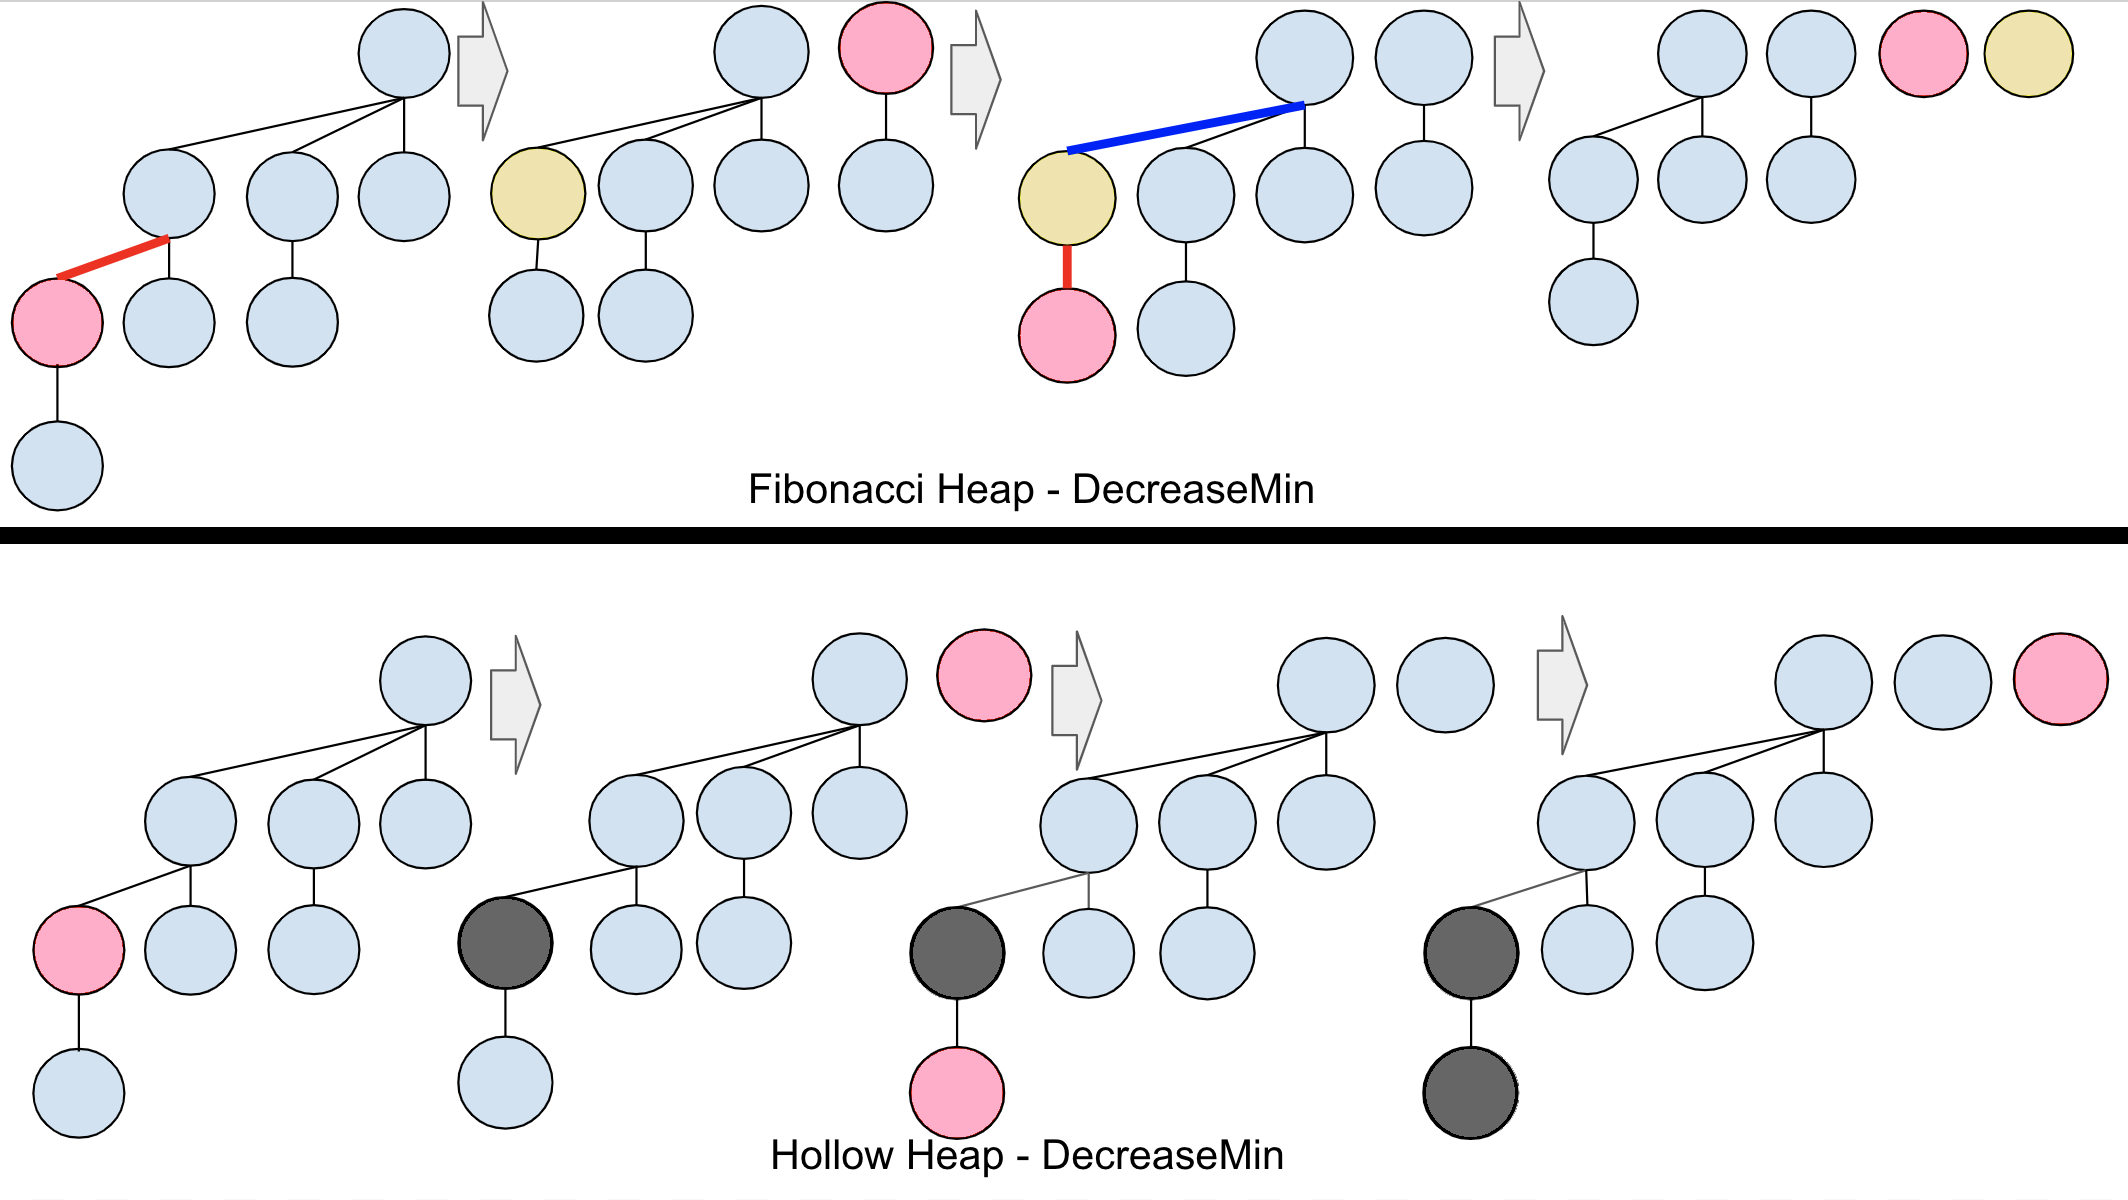
\includegraphics[scale=0.15]{figures/HollowHeaps-DecreaseKey-Comparsion-new.png}
    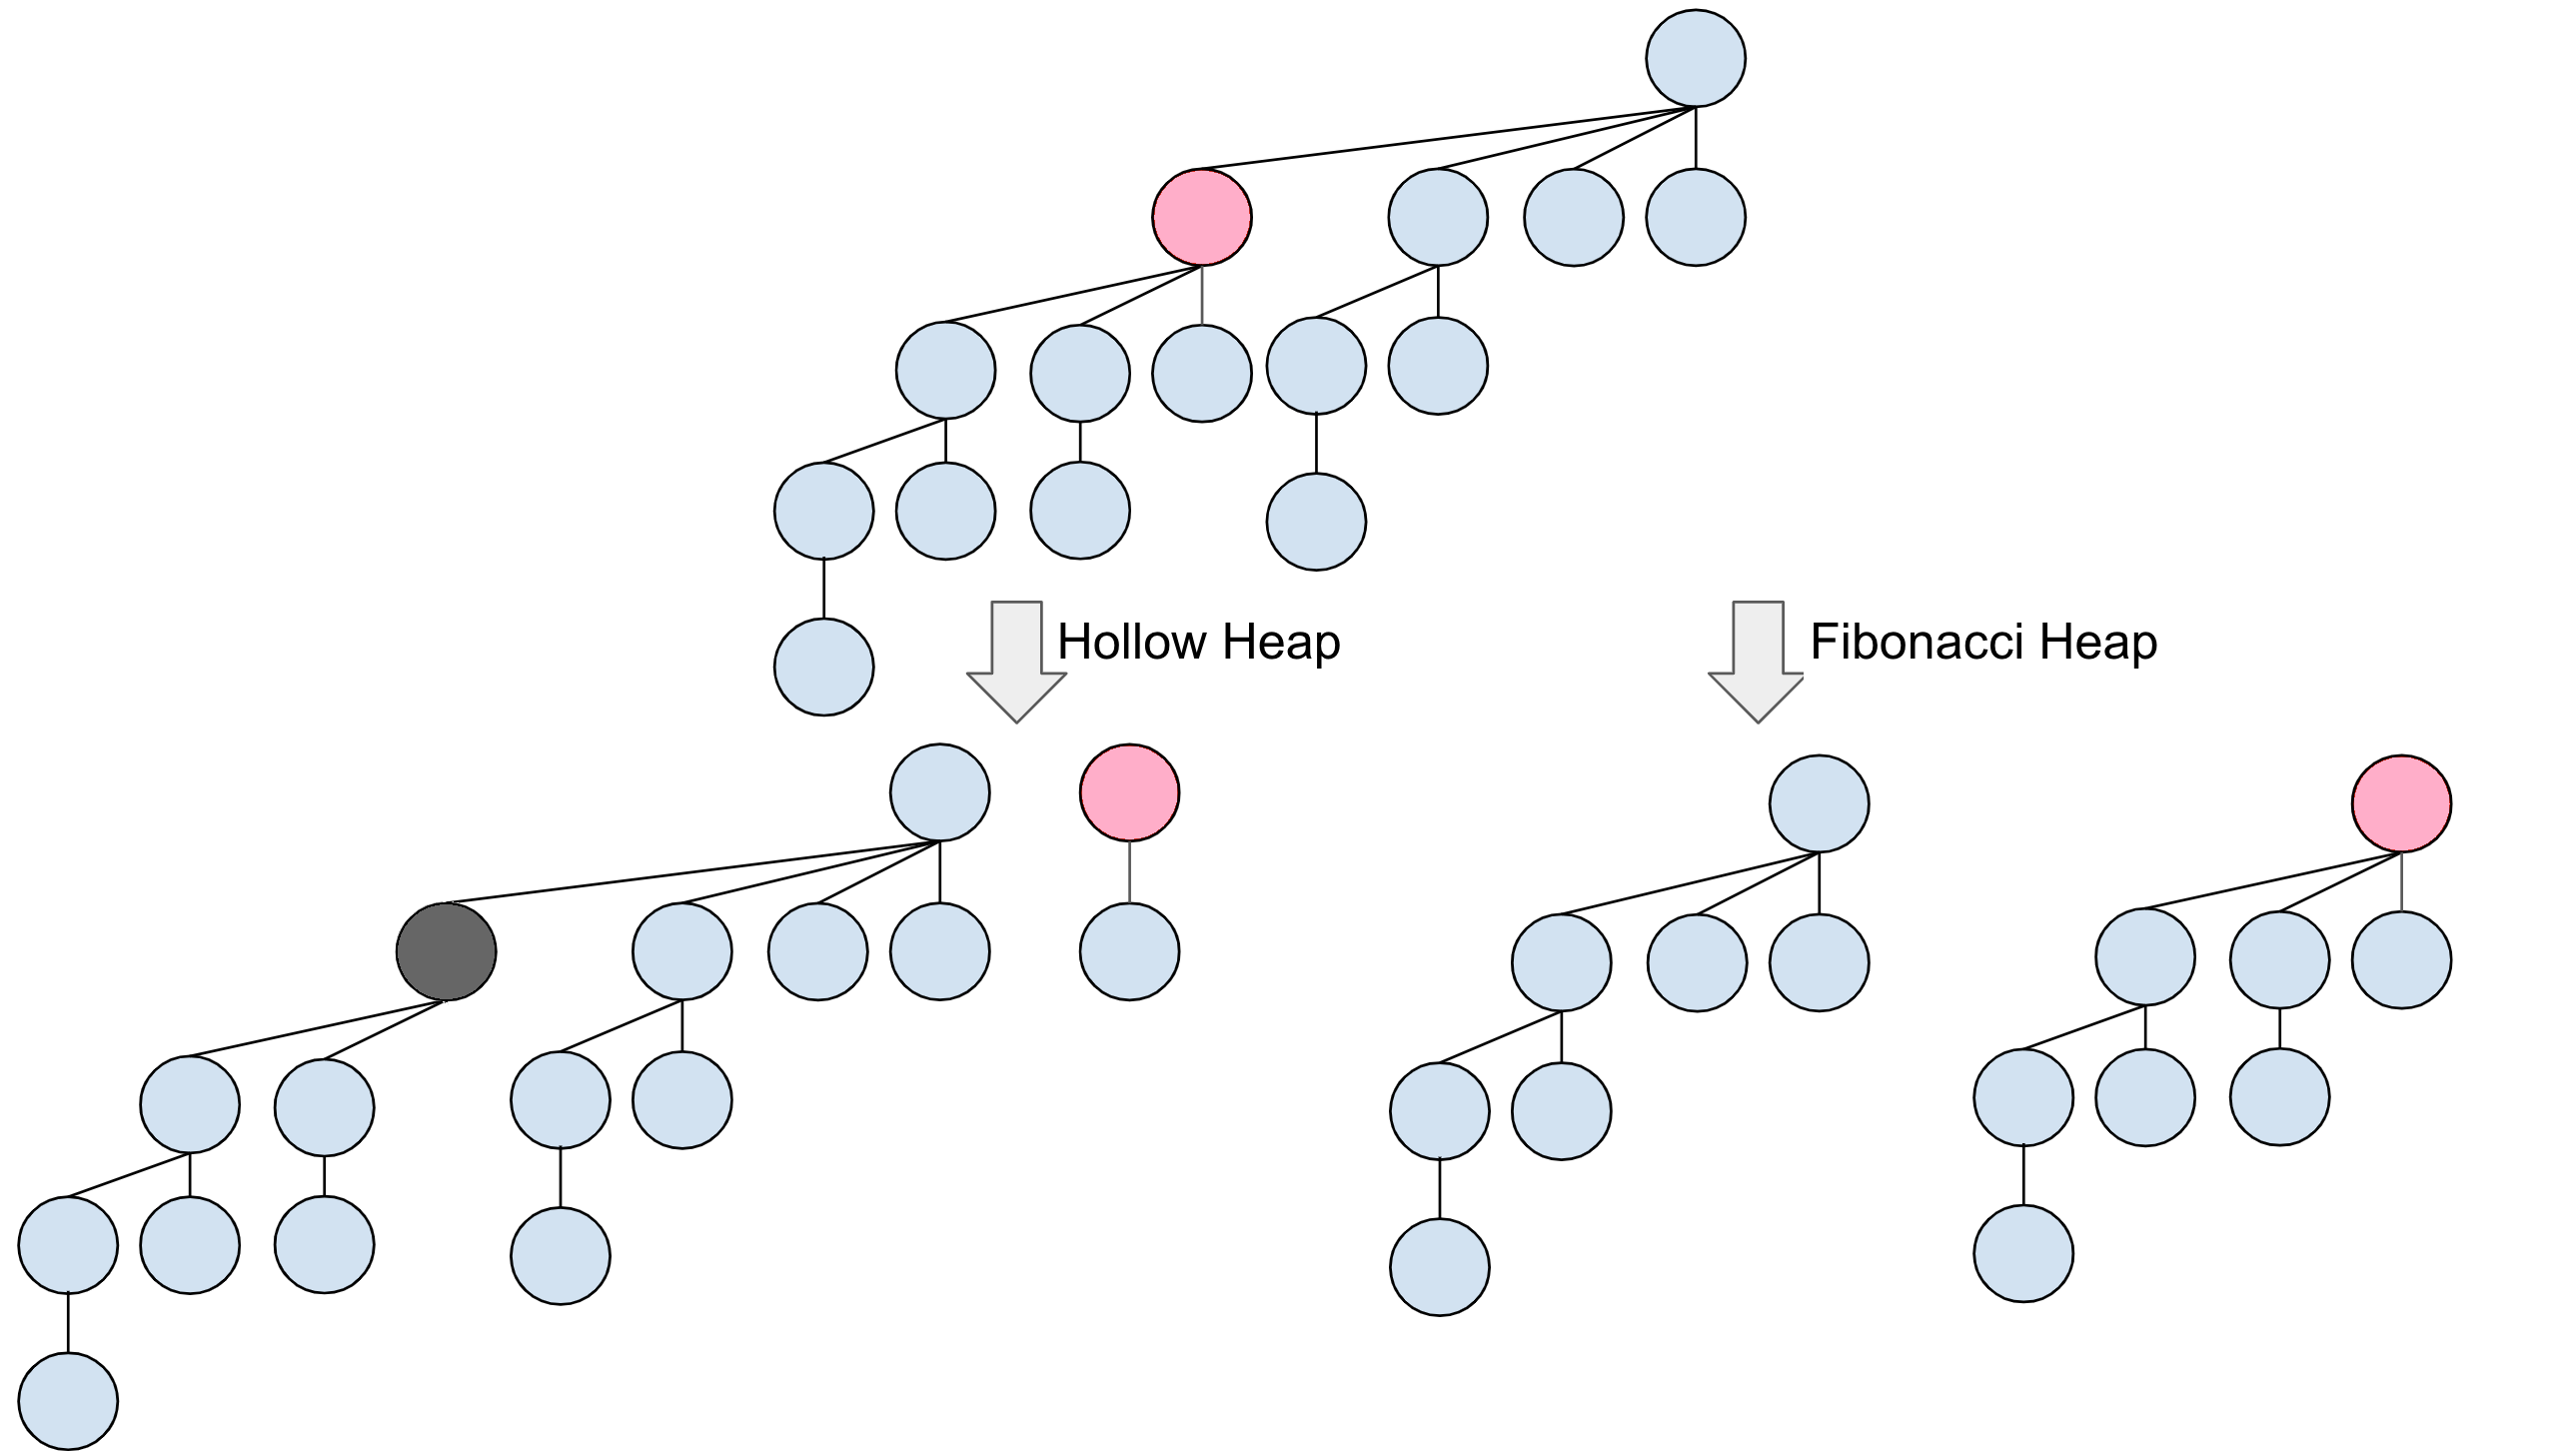
\includegraphics[scale=0.15]{figures/HollowHeaps-DecreasKey-SecondExample-new.png}
    \caption{This diagram shows a side-by-side comparison of the \texttt{DecreaseKey} operation in Hollow Heaps vs Fibonacci Heaps. Marked nodes are yellow, whereas hollow nodes are gray. We note that the Hollow Nodes preserve the structure of the original tree, and also mark points where future cuts must be made. In the top diagram, we first decrease the key of a node (pink), and then decrease the key of its child (pink) and show this effect on Fibonacci Heaps as well as Hollow Heaps. In the bottom diagram, we show the effect of \texttt{DecreaseKey} on a node with $>2$ children (pink) for both Fibonacci Heaps and Hollow Heaps.}
    \label{fig:DecreaseKeyHollowHeapFibHeapComparsion}
\end{figure*}

%%%%%%%%% END: SECTION COVERING DecreaseKey %%%%

%%%%%%%%% BEGIN: SECTION COVERING ExtractMin %%%
\subsection{The New \texttt{ExtractMin}}
\label{subsec:delete_min}
Now that we've modified \texttt{DecreaseKey} to essentially avoid the work introduced by \textit{cascading cuts} by marking future cuts, we need to actually make the cuts (by removing the hollow nodes).

The most natural place to do this is during the \texttt{ExtractMin} operation. Other operations, such as \texttt{Meld}, \texttt{Insert}, and \texttt{FindMin} already have worst-case (\textbf{not} amortized) run-times of $O(1)$, meaning that the amount of \textit{actual} work we can do during these operations is limited. On the other hand, \texttt{ExtractMin} is already tasked with performing significant clean-up work by joining trees. As such, we take advantage of this operation to get rid of some of the hollow nodes.

We modify \texttt{ExtractMin}$(Q) \rightarrow k$ to do the following:

\begin{enumerate}
    \item Remove the item containing the minimum node, and add its of each children as new trees in the heap.
    \item While there is a hollow root, destroy that root and make each child into its own root. Repeat this process until all of the roots are full.
    \item Link together roots of the same rank, increasing the rank of the node with the lower key and breaking ties arbitrarily.
\end{enumerate}

For an example of this function, see Figure \ref{fig:delete_min_hollow_heap}.

The amortized runtime of this operation is $O(\log N)$, where N is the total number of nodes in the tree. We will discuss calculating the amortized runtime of this operation in a later section.


\begin{figure*}
    \centering
    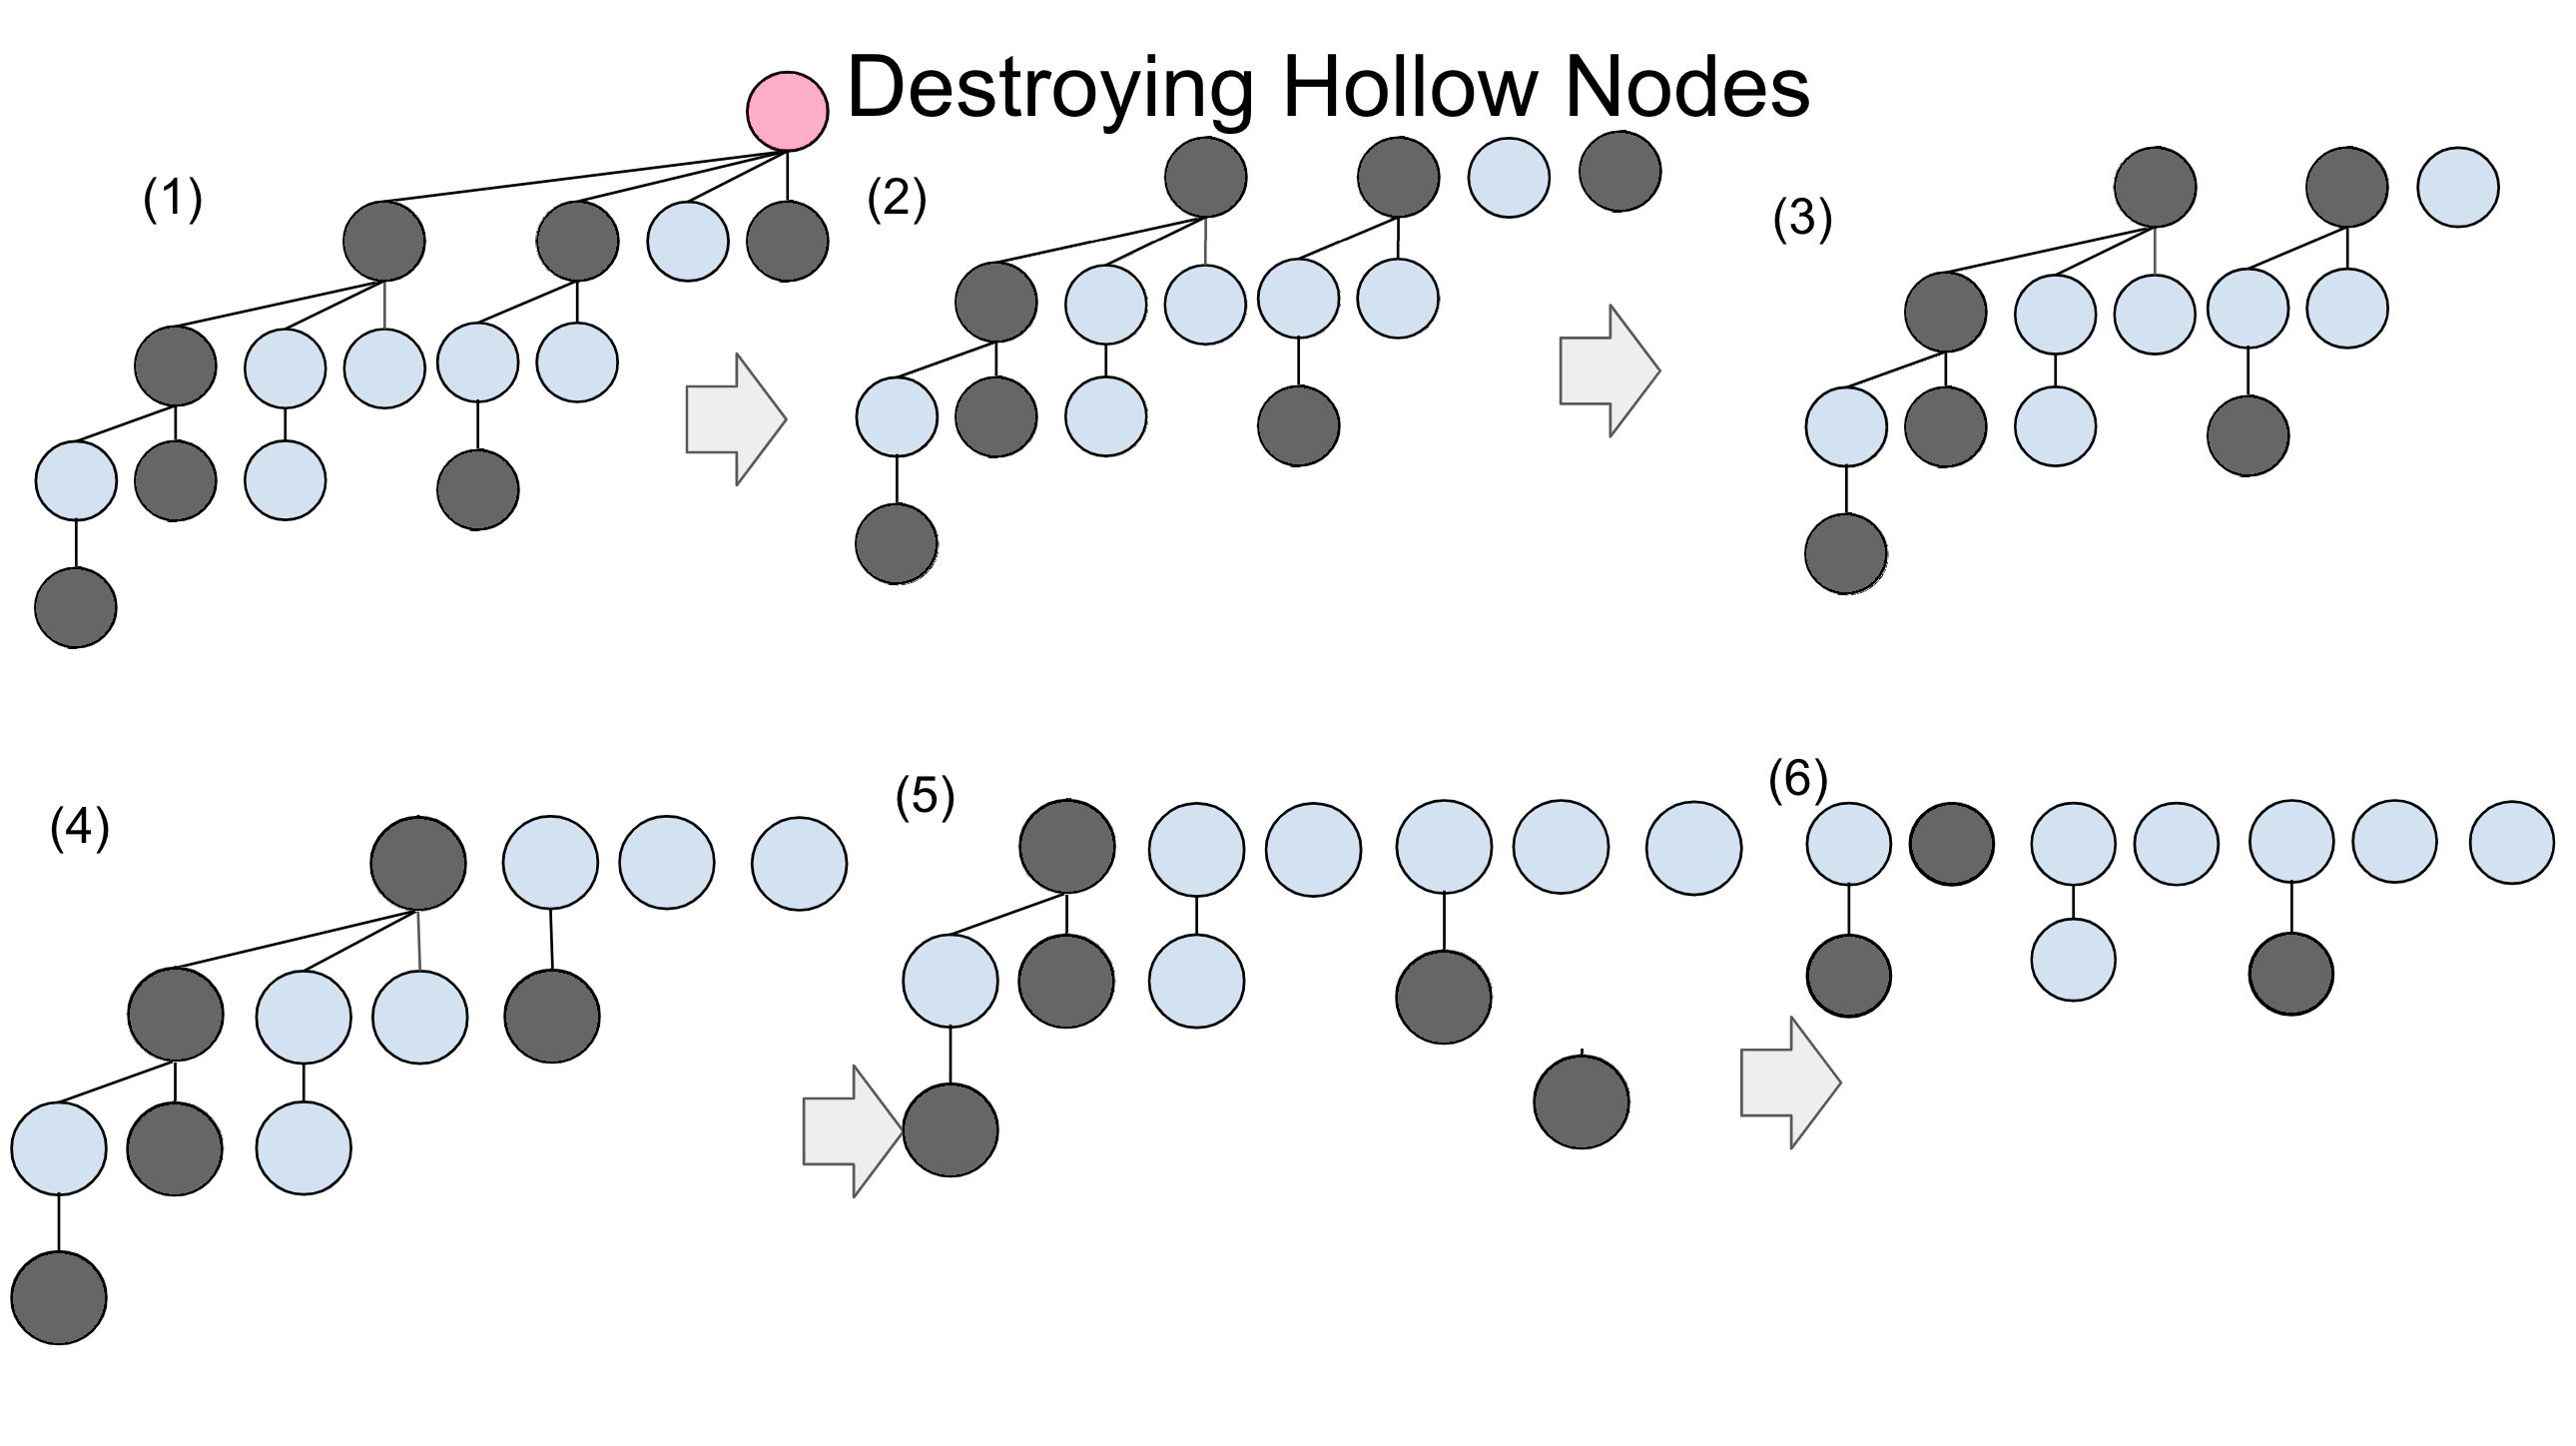
\includegraphics[scale=0.15]{figures/DestroyingHollowNodes-new.png}
    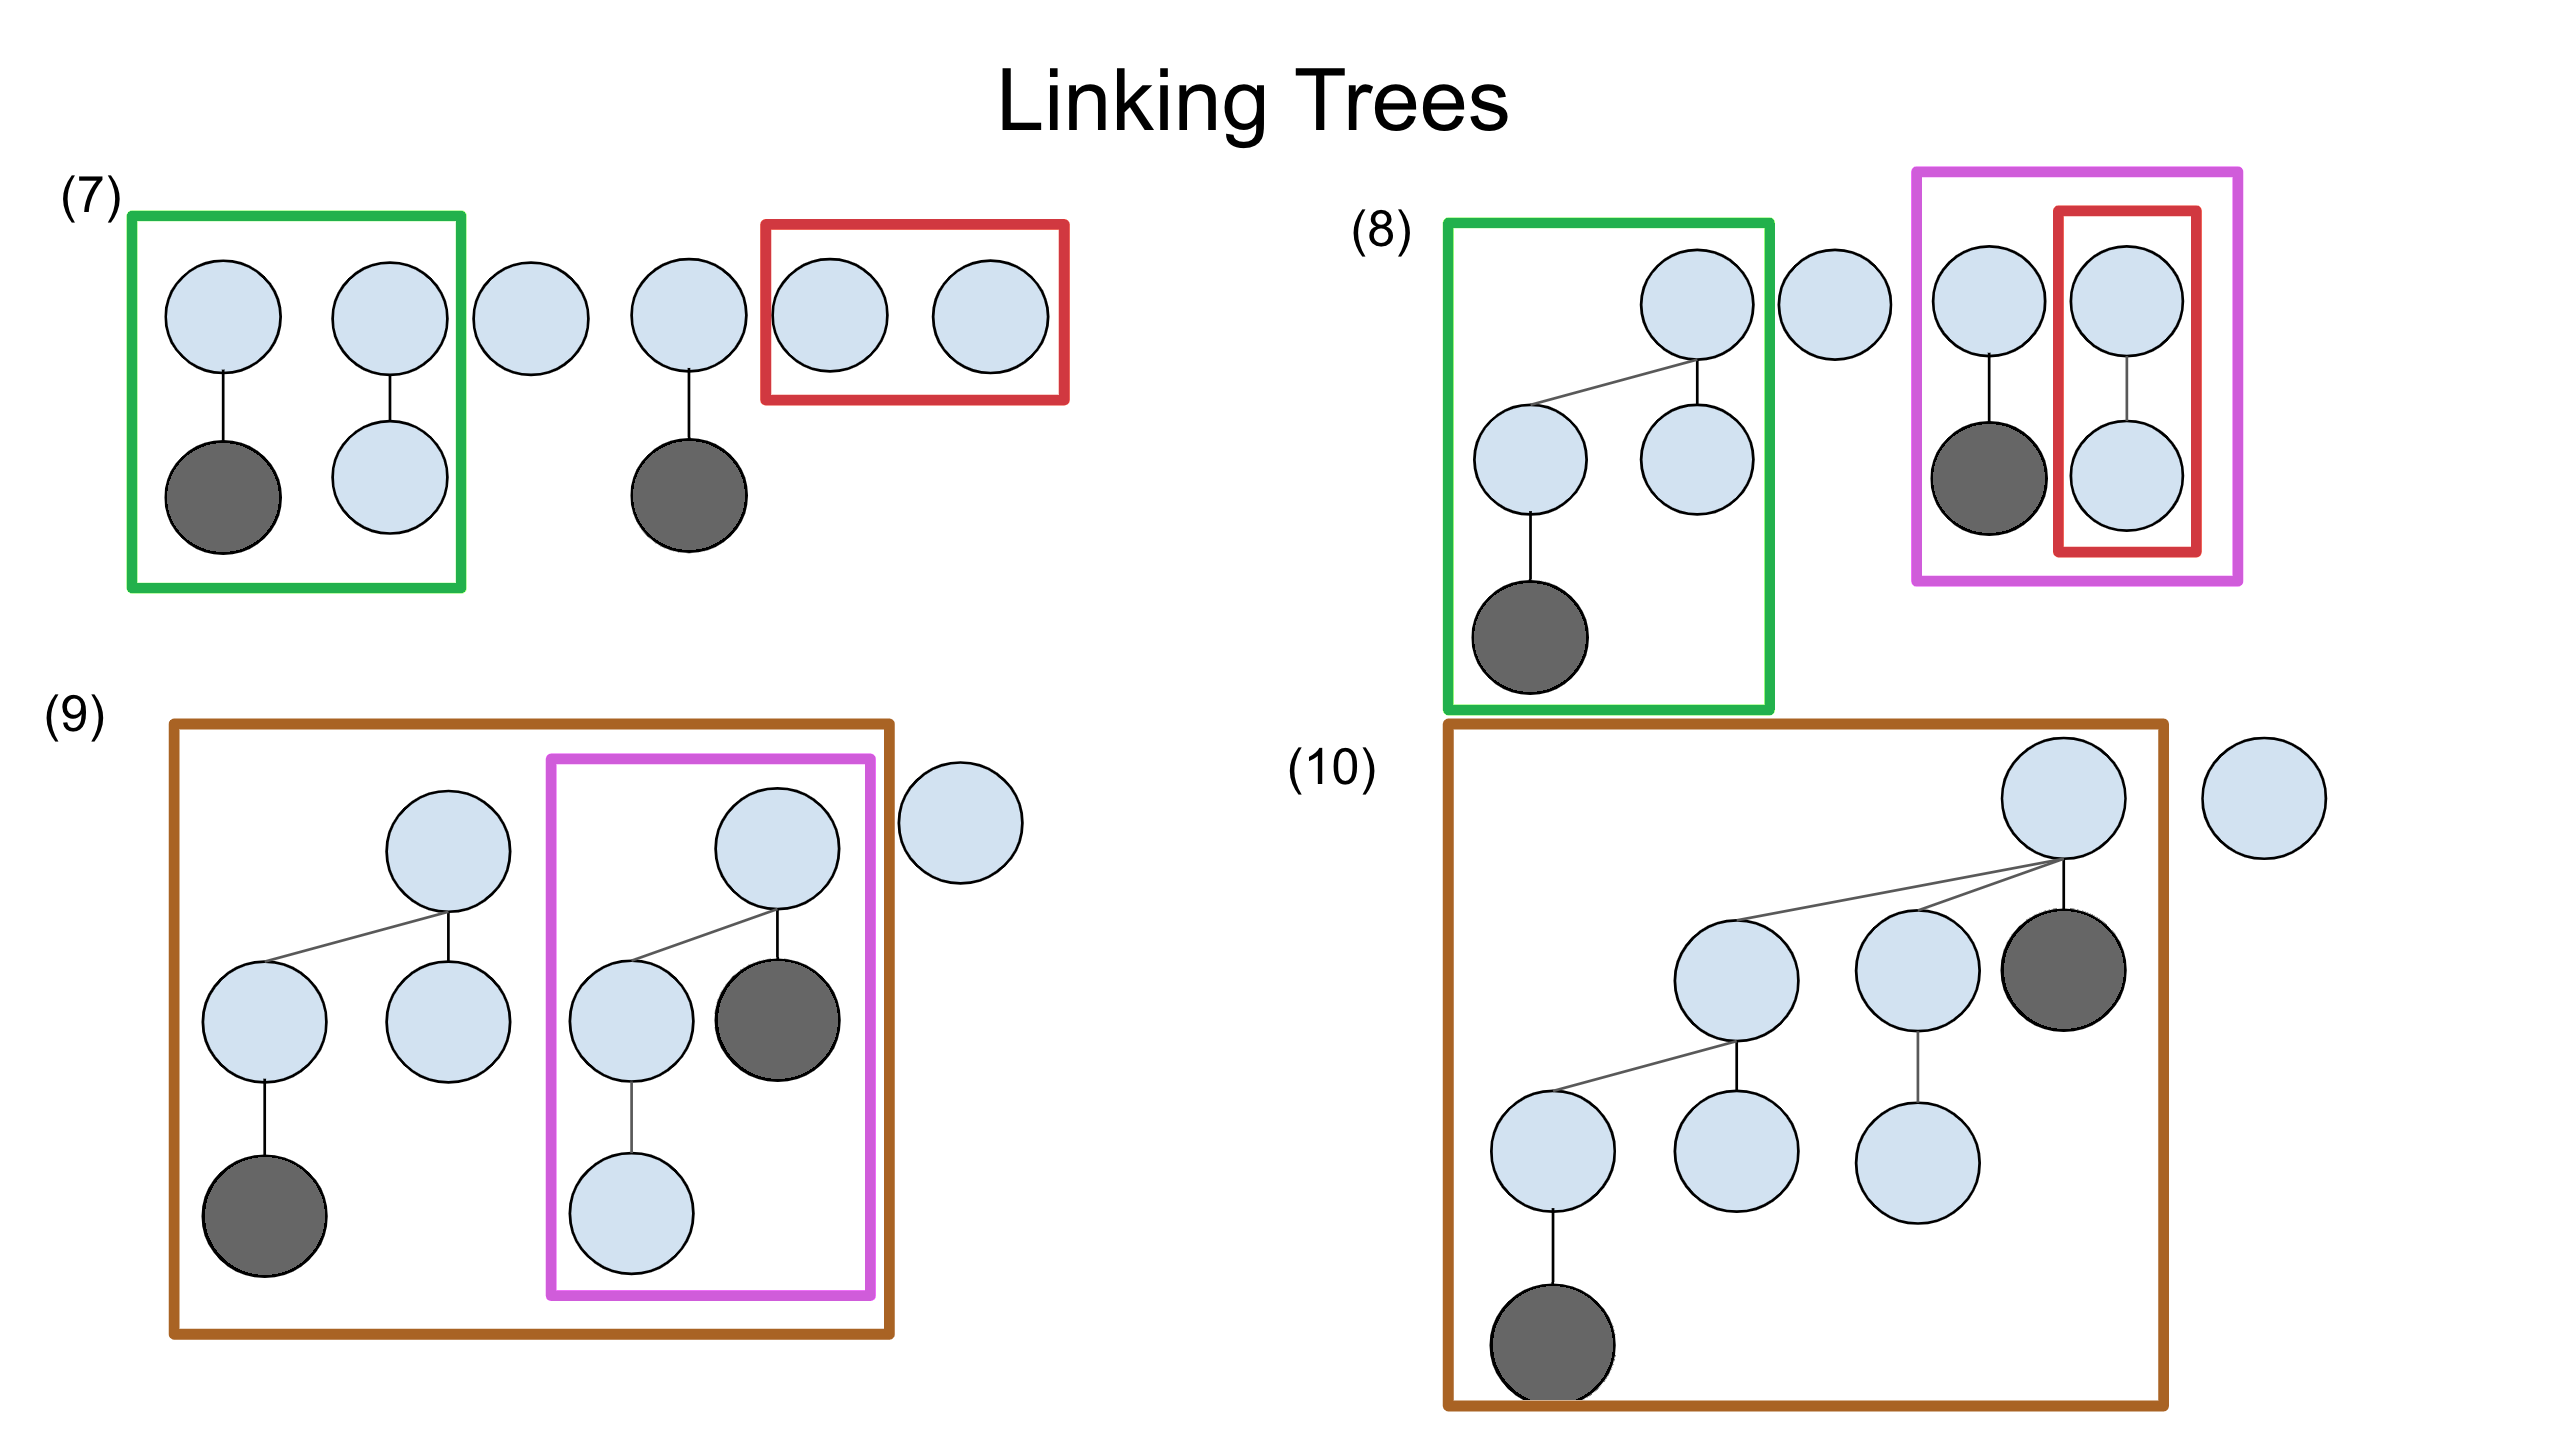
\includegraphics[scale=0.15]{figures/LinkingTrees-new.png}
    \caption{In this diagram, we show the sequence of steps which occur when an \texttt{ExtractMin} operation is carried out. Hollow nodes (gray) already exists throughout the tree. $(1) \to (2)$ deletes the minimum node from the heap and adds its children sub-trees as new trees. $(2) \to (6)$ shows the process of removing hollow nodes (gray) which becomes roots, and doing this until now hollow roots remain. $(7) \to (10)$ how the process of linking same-rank nodes until only nodes of distinct rank remain.}
    \label{fig:delete_min_hollow_heap}
\end{figure*}

%%%%%%%%% END: SECTION COVERING ExtractMin %%%%

\subsection{Other Operations}
\label{subsec:other_operations}
The other operations \texttt{Meld}, \texttt{Insert}, \texttt{FindMin} are essentially identical to their Fibonacci Heap counterparts. We recall from Fibonacci Heaps that each of these operations has an $O(1)$ amortized and worst-case run-time.


\subsection{Summary of the Data Structure}
\label{subsec:correctness}
Above we've presented a modified version of Fibonacci Heaps motivated by two key ideas: (1) we can be lazier during the \texttt{DecreaseKey} operation to achieve worst-case $O(1)$ time-bounds while maintaining the same amortized run-time for other operations, and (2) we can simplify the presentation of \texttt{cascading cuts} by instead introducing \texttt{hollow nodes}.

It is worth noting that, because the tree contains some number of hollow nodes in addition to n nodes for each element, we can no longer assume the maximum rank of a given node is no more than $\log n$. Instead, we consider the tree in terms of N, where N is the total number of full and hollow nodes in the tree. We prove below that the run-time of \texttt{ExtractMin} is amortized $O(\log N)$, which for a sufficiently large number of hollow nodes may be $\omega(\log n)$. We discuss how to rebuild the heap and mitigate this difference below.\footnote{Note that in common applications of Priority Queues, such ask common graph algorithms like Dijkstra's or Prim's, this limitation only leads t a constant factor increase in run-time since $N = \Theta(\#\text{edges} + \#\text{vertices)} = O(n^2) \implies O(\log N) = O(\log n)$}

\section{Rank Invariant \& Runtime Justification}
\label{sec:invariant_justification}

First, we'll show that the rank invariant given above is a legal invariant. Next, we will explain why it helps us maintain our amortized runtime.

\subsection{Legality}
\label{subsubsec:legality}
First, we can ensure that this invariant works with the Heap Invariant we carried over from Fibonacci heap- namely, that every node of rank r contains at least $F_{r+3} - 1$ descendants. For the full nodes, this applies as it would for Fibonacci heap, since each node with a rank $r$ has $r$ children that follow the Heap Invariant. If the node is hollow, it either contains 0 children, one child of rank 0 (in which case the invariant holds trivially), or it contains two children of ranks $r-1$ and $r-2$, and so the invariant holds because $F_{r+2} + F_{r+1} = F_{r+3} \geq F_{r+3} - 1$.

From this we also know that the rank of any given node is at most $log_{\phi}N$, where N is the number of nodes. Note that this is slightly different from Fibonacci heaps, because instead of just having $n$ nodes, we have $n$ nodes and some number $z$ hollow nodes. Therefore, N in this case is equal to $n + z$. However, we can still perform our analysis in terms of $N$.

\subsection{Run-time Justification}
\label{subsubsec:run-time}
Next, we show that the amortized time per multi-root hollow heap runs in amortized cost $O(log N)$ for \texttt{ExtractMin} on a heap of $N$ nodes, and $O(1)$ for all other functions. We can define our potential function to be the number of full nodes without full parents (i.e. all roots and full children of hollow parents). Intuitively we can think of this as the 'mess' creating by both lazy melding and keeping hollow nodes with some children in the tree, which we clean up in ExtractMin. We'll go through each operation (note that the real runtime is based on the number of links being made).\\
\texttt{Insert} has a constant real cost $O(1)$, and we're adding one new root, so the amortized cost is $O(1) + 1 = O(1)$\\
\texttt{FindMin} and \texttt{Meld} also have costs of $O(1)$, and the number of roots and full nodes of hollow parents doesn't change, so the amortized cost for both $O(1) + 0 = O(1)$\\
In \texttt{DecreaseKey}, the real cost is $O(1)$, and because of our rank invariant, we know that we'll create one new root and there will be at most 2 additional full children on the newly created hollow node.  $O(1) + 3 = O(1)$\\
In \texttt{ExtractMin}, every link converts a full root into a full node with a full root parent, so while linking $l$ times is $O(l)$, the change in potential decreases by $l$, so the amortized cost for those operations is 0. However, the delete function itself can cause the potential to increase by the number of children of the root (because each of these children become roots themselves), which is a maximum potential increase of $\log N$. Therefore, the amortized runtime of \texttt{ExtractMin} is $O(1) + \log N = O(\log N)$.

Something interesting to note is that the number of children being two only increases the amortized cost of decrease-key by a constant amount. Because of this, instead of hollow nodes retaining at most two children, we could have them retain any constant number of children and the operations above hold, Although the amortized cost of decrease-key will increase by a constant amount.

\section{Incorrect Hollow Heap Variants}
\label{sec:other_hollow_heap_variants}
It may be unclear why we have to keep at most a constant number of children for each hollow node. The intuitive reason is that keeping at most $c > 1$ nodes keeps the trees relatively balanced. Otherwise, we could create degenerate trees, where each iteration of the operations for the degenerate tree requires more work than amortized cost can make up for. We have provided a few such examples for three seemingly valid alternatives to the rank invariant given above.

\subsection{Variant 1 - Let hollow nodes keep all of their children:}
\label{subsubsec:variant1}
\begin{figure*}
    \centering
    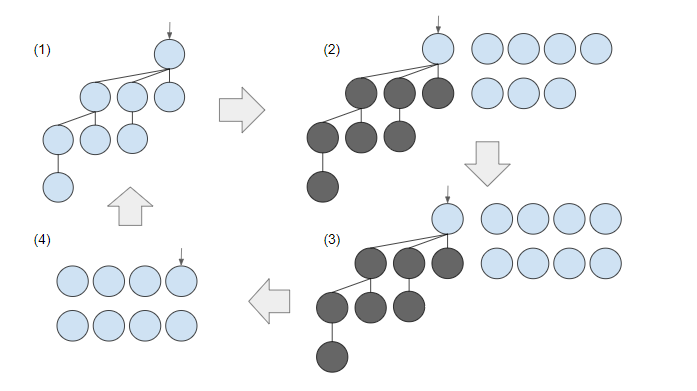
\includegraphics[scale=0.75]{figures/variant_1.png}
    \caption{These images show the iterations of the first degenerate example. $(1) \to (2)$ calls decrease key on all of the nodes in the tree. $(2) \to (3)$ inserts one more node in the heap. $(3) \to (4)$ performs the first half of extract-min, which deletes the minimum node as well as all of the hollow nodes. $(4) \to (1)$ performs the second half of extract-min by melding all of the nodes together.}
    \label{fig:variant_1}
\end{figure*}
The issue here is that you could have a full tree made up almost entirely of hollow nodes, which leads to a very expensive \texttt{ExtractMin}. To see this, build up a full tree with a rank of $r$ with $n$ elements. call decrease-key on all of the elements in the tree, converting every node in the original tree except the root to a hollow node and creating $(n-1)$ new one-node roots. Add one more non-minimum node, resulting in $n$ additional roots with one element. Call extract-min. This results all of the elements in the original tree being deleted and all of the single element roots being linked together. The final result will be a tree equivalent to the original full tree with a rank $r$. An example of this is provided in Figure \ref{fig:variant_1}.We can repeat this process an arbitrarily large number of times.\\
Each of the iterations will require one \texttt{ExtractMin}, but that \texttt{ExtractMin} will require $O(r^2)$ operations to delete all of the hollow nodes and merge all of the single-node roots. Even if all other operations had a cost of 0, we have $O(r)$ total operations for each iteration, and the total runtime will be lower-bounded by $O(r^2)$, which is higher than the desired runtime $O(r)$.

\subsection{Variant 2- Do not allow hollow nodes to have any children:}
\label{subsec:variant2}
\begin{figure*}
    \centering
    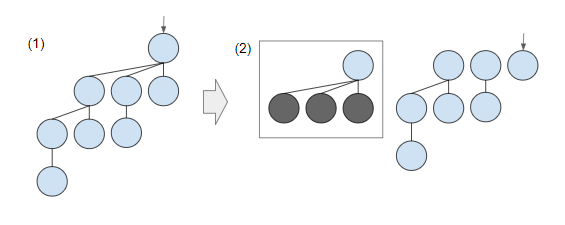
\includegraphics[scale=0.75]{figures/variant_2.png}
    \caption{These images show the second degenerate example. $(1) \to (2)$ calls decrease key on all of the children of the root. The boxed tree is the tree we are interested in for our analysis.}
    \label{fig:variant_2}
\end{figure*}
With this we can create a degenerate case that violates the heap invariant. Suppose we had a full tree of rank r (we can generate this by inserting $n+1$ nodes and calling one extract-min.) Next, we can decrease the key for each of the children, where all of the new values are less than the original minimum and the values decrease with the rank of the original child. The result is that the original tree will contain a node of rank $r$ and $r$ hollow nodes of rank 0. An example of this is provided in Figure \ref{fig:variant_2}. We could recursively call a series of extract-min and decrease key for the smaller trees until only the tree of rank $r$ remains, but this is not necessary for our analysis.

This tree violates one of our invariants, as our root has a rank $r$ but the number of descendants it has is $r$, which less than $F_{r+3} - 1$. This is similar to the type of degenerate cases we try to avoid using cascading cuts in Fibonacci heap; we are cutting off large portions of the tree without maintaining a balancing structure in the tree.

\subsection{Variant 3- Allow hollow nodes to have at most one child:}
\label{subsec:variant3}
\begin{figure*}
    \centering
    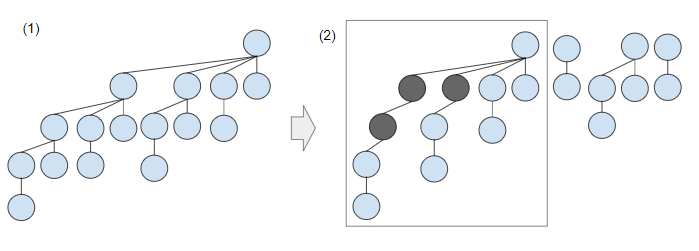
\includegraphics[scale=0.75]{figures/variant_3.png}
    \caption{These images show the third degenerate example. $(1) \to (2)$ calls decrease key on every node that has more than one child. The boxed tree is the tree we are interested in for our analysis.}
    \label{fig:variant_3}
\end{figure*}
Once again, we can potentially create degenerate trees with this approach. Suppose we had a full tree of rank $r$. For every node with two children or more, decrease the key, resulting in at most one child for every node. In this case, each child of the root with rank $x$ will have $x-1$ descendants.  An example of this is provided in Figure \ref{fig:variant_3}.
This also violates the heap invariant, because the total number of descendants will be $r(r-1)/2$, and $r(r-1)/2 < F[r+3]-1$ for any $r > 0$.

\section{Single-Root Hollow Heaps}
One interesting aspect to note when analyzing Hollow Heaps is that there is information in a significant number of comparisons during \texttt{Insert}s that could potentially be utilized. A technique orthogonal to hollow nodes can be applied where all of the elements in the heap share one common root. (Note that this version of Hollow Heaps borrows especially heavily from the one-root Fibonacci Heap.\cite{FibHeapsRevisited}. While that data structure is not the focus of our paper, we will provide details of the properties of one-root Fibonacci Heaps as they apply to one-root hollow heaps.)

In the spirit of caching, it's possible to make use of the existing tree structure to ``cache'' these comparisons. We do this by introducing the concept of ``unranked'' links.

\begin{defn}
    A \textit{ranked} link is a link operation which occurs between two nodes of equal rank, $u$ and $v$. The node with the smaller key (ties broken arbitrarily) becomes the parent, and it's rank is increased by $1$. This is the same as the link operations we saw in multi-root Hollow Heaps and Fibonacci Heaps.
\end{defn}

\begin{defn}
    A \textit{unranked} link is a link operation which occurs between two nodes of \textit{different} ranks, $u$ and $v$. The node with the smaller key (ties broken arbitrarily) becomes the parent. The ranks of the two nodes remain unchanged. This \textit{unranked} link simply serves as a way to cache previous comparison operations.
\end{defn}

\textit{Unranked} links are created primarily during \texttt{Meld} operation when the (single) roots of the two heaps are compared and linked together (if the roots have distinct ranks, we do an \textit{unranked} link; if not, we do a \textit{ranked} link).

Otherwise, we mainly don't bother with unranked links. We ignore them during the child-movement process, and maintain only the following rank invariant, which is nearly identical to our original rank invariant:

\begin{defn}
A node $u$ of rank $r$ has exactly $r$ \textit{ranked} children, of ranks $0,1, \cdots, r - 1,r$ unless $r > 2$ and $u$ was made hollow by a decrease-key, in which case $u$ has exactly two \textit{ranked} children, of ranks $r - 2$ and $r - 1$. (A node can have any number of unranked children.)
\end{defn}

We note that the proofs of correctness are essentially the same as those used for the multi-root hollow heap. Similarly, the unranked link component has no impact on the run-time analysis, since unranked links do not change the real runtime of each operation and are not part of the potential function for one-root hollow heaps.

\section{Two-Parent Hollow Heaps}
\label{sec:two-parent}
Continuing with the idea of trying to minimize the amount of work done as much as possible, we can reduce number of pointer transfers by relaxing the constraint that our heap must be a tree. In other words, if we relax the restriction that our heap is a tree, we can be even lazier and not move the elements in our hollow node at all when we decrease a key.

Instead, we can allow DAGs (Directed A-cyclic Graphs) to take the place of trees. In the \texttt{DecreaseKey} operation, rather than moving the top two children from the newly hollowed node $u$ to the newly created node $v$, we simply make $v$ a parent of $u$. See Figure \ref{fig:two-parent-hollow-heap-decrease-key} for an example of this.

Because we only add a second parent when a node becomes hollow, it follows that a full node can have at most one parent if it's full and at most two parents if it's hollow. If a parent has a child formed from \textit{DecreaseKey}, it is called a virtual parent. A parent's virtual children is the number of children it gained from links (think of these as 'traditional' children) plus the number of children it gained from nodes being hollowed out. The rank of the virtual parent is equal to the rank of the hollow node it became a virtual parent of minus 2, or 0 if the rank of the hollow node was less than 2.

\subsection{\texttt{DecreaseKey}}
\label{subsec:decrease_key_DAG}

\begin{figure*}
    \centering
    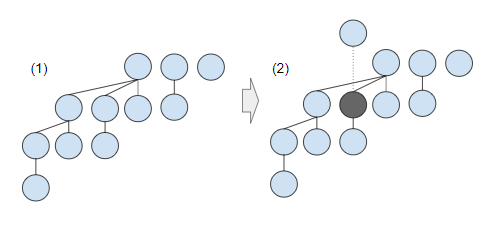
\includegraphics[scale=0.75]{figures/2Parent_decreaseKey.png}
    \caption{We perform a \texttt{DecreaseKey} operation on a node in a Hollow Heap that allows for two-parents. No children are moved, and instead the newly decreased node becomes a virtual parent of the newly hollowed node (in gray).}
    \label{fig:two-parent-hollow-heap-decrease-key}
\end{figure*}

As stated before, when we decrease a key in a two-parent hollow heap, we don't transfer any of the children. Instead, we create a node with the new key value and make the new node a virtual parent of the old node. Figure \ref{fig:two-parent-hollow-heap-decrease-key} contains an example of this. Once again, we maintain an invariant that is nearly identical to our original rank invariant.
\begin{defn}
A node $u$ of rank $r$ has exactly $r$ \textit{virtual} children, of ranks $0,1, \cdots, r - 1,r$ unless $r > 2$ and $u$ was made hollow by a decrease-key, in which case $u$ has exactly two \textit{virtual} children, of ranks $r - 2$ and $r - 1$.
\end{defn}

\subsection{\texttt{ExtractMin}}
\label{subsec:extract_min_DAG}

\begin{figure*}
    \centering
    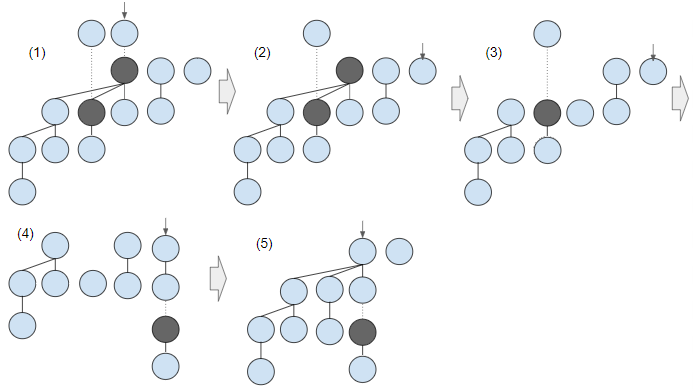
\includegraphics[scale=0.75]{figures/2Parent_extractMin.png}
    \caption{We perform an \texttt{ExtractMin} operation on a two-parent hollow node, where gray nodes are hollow nodes and the dotted lines are their virtual parents. $(1) \to (2)$ deletes the current min.  $(2) \to (3)$ destroys the new hollow root. Note that its hollow child is not destroyed, because it has a virtual parent. $(3) \to (4)$ links together two elements, one of which contains the hollow nodes as a virtual child, and $(4) \to (5)$ link the remaining roots.}
    \label{fig:two-parent-hollow-heap-extract-min}
\end{figure*}

Like one-parent hollow heaps, we perform \texttt{ExtractMin} by deleting the minimum node, destroying any roots which are hollow, and melding the remaining trees together. However, there are two important things to keep in mind. First, nodes with virtual parents are not considered roots, because roots do not have parents. Therefore, even if a hollow node's only remaining parent is a virtual parent, it is not destroyed. Furthermore, the rank of a virtual parent depends on the rank of the hollow node it was made a parent of. This can influence what roots that node can link with during the melding stage. See Figure \ref{fig:two-parent-hollow-heap-decrease-key} for an example of \texttt{ExtractMin}.


\section{Reconstruction}
One of the major drawbacks of Hollow Heaps is the fact that the amortized run-time for \texttt{ExtractMin} is $O(\log N)$ instead of $O(\log n)$. The run-time is a function of the number of nodes in the heap, both full and hollow, which can be arbitrarily large. In fact, we have the following Lemma:

\begin{lem}
It is possible to create a Hollow Heap with an arbitrary number of nodes. This means that $N$, the number of nodes, can be arbitrarily larger than $n$, the number of elements.
\end{lem}

\begin{proof}
Assume we have $n$ full nodes in our heap. Without any optimization, every \texttt{DecreaseKey} operation increases the number of hollow nodes by $1$ and the number of full nodes by $1$. As such, we can create a Hollow Heap with $m+n$ nodes, where $m$ is arbitrarily large, and $n$ full nodes by performing \texttt{DecreaseKey} on a node that isn't a child of a root node, extracting the minimum (setting the number of full nodes back to $n$), and repeating this process $m$ times.
\end{proof}

In order to avoid this drawback, the simplest solution is to force $N$ to be $\Theta(n)$. Simply put, when $N > cn$ for some constant $c > 1$, rebuild the entire heap. To do this, we destroy every hollow node in the tree, reduce every other node to n one-element roots, and link all of the roots together. Rebuilding the entire heap will take $O(N)$. However, we only rebuild after $(c-1)n$ hollow nodes have been added to the data structure. Therefore, using the banker's method, we can add a cost of 2 for every hollow node that is added (adding a hollow node costs O(1), so this amortized cost is still $O(1)$). By the time we rebuild the heap, we will have accrued $2(c-1)n$ credit, and our amortized cost will be $cn - 2(c-1)n = 0$.

\section{Interesting Component: Reducing Hollow Nodes}
\label{sec:interesting_componebt}
A practical way to reduce the ratio of hollow nodes to full nodes, thereby reducing the number of times reconstruction must be called, would be to reduce the number of hollow nodes that fill the tree in the first-place. We propose and analyze a few mechanisms through which this can be accomplished, making clear that most mechanisms are not strictly better, but rather offer trade-offs for the data structure.

\subsection{Cutting Hollow Leaves}
One fairly simple way to reduce the number of hollow nodes $N - n$ is that whenever \texttt{DecreaseKey} is used on a leaf node, we create a new root node as usual but destroy the old leaf node instead of hollowing it. Such an optimization saves a constant amount of work from an eventual \texttt{ExtractMin} by avoiding a check on whether the node is hollow when it would otherwise be raised to the root list.
Note that this does not fix the disparity between full nodes and hollow nodes in the worst case, as we could still perform the operations above as described in the proof and simply not reduce the key of any leaf nodes. Furthermore, we need to decrease the rank of the parent to achieve this, so we would need to maintain pointers to each of the parent nodes. However, we have to check the children during this step anyway, so the only additional work is to remove the child and decrease the rank of the node's parent by one.
\subsubsection{Extension - Hollow leaf chains}
One potential extension of this is to perform "chains" of deletion. Namely, if you delete a hollow leaf, it may result in another hollow leaf. You could continue deleting these chains of hollow leaves, reducing the number of hollow leaves by some amount $i$ rather than by 1 for a given DecreaseKey. 
Note that this could result in fewer hollow nodes; namely, we would cap the number of hollow nodes as being less than or equal to N - (the number of roots + the number of leaves in the hollow heap trees), which is a tighter bound than what we had before. However, we run into the same worst-case scenario where if we decrease keys and extract minimums without ever reducing the key of leaf nodes or root child nodes, the number of hollow nodes becomes arbitrarily large. Furthermore, while this doesn't increase the amortized amount of work we have to do, we are ultimately just transferring some of the work in \texttt{ExtractMin} back to \texttt{DecreaseKey}, and we still have to maintain the additional information of the parent for each node in the heap. 

% Possibly discuss how hollow heaps in most algos still have O(log n) time (eg, the N is not really a big deal in terms of run-time). 

%%commenting out for now, because the results may not be substantial enough
%\subsubsection{Avoid Hollow Node Creation When Possible}
%An aspect not discussed explicitly in the Hollow Heaps paper \cite{HollowHeapsIntro} has to do with the fact that we avoid hollow node creation if the \texttt{DecreaseKey} operation doesn't violate our heap invariant (See Section \ref{subsec:correctness} for a discussion). This means that the number of hollow nodes increases only with the number of \texttt{DecreaseKey} operations which lead to an invariant violation. 

% Consider proving that with a large key-space, the # of invariant violations should be small (depends on distribution of keys)
% Letting $K$ b
\subsection{Node Revival}
Another approach we can take at this point is to attempt to \texttt{minimize} the number of Hollow Nodes in the tree by reusing hollow nodes as full nodes.

One approach we consider is the relaxation of the constraint in \cite{HollowHeapsIntro} that ``Hollow nodes may never become full.'' We observe that in inserting a new key, or decreasing the key of an existing node, we can avoid creating a new node in the root of the tree and eliminate a hollow node by finding a suitable hollow node and \textit{resurrecting} it.

\subsubsection{Exact Resurrections}
We could define ``suitable'' as hollow nodes with the same key as that of the node we are trying to insert, or that of the new key we are trying to decrease an existing node to. Such a definition, along with the constraint of sustaining the $\bigo{1}$ run-time complexities of \texttt{Insert} and \textit{DecreaseKey} intuitively leads to maintaining a hash table mapping keys to hollow nodes with that key. Under this setup, \texttt{Insert} is modified to first perform a look-up into the hash table. If the look-up returns a match, the first node in the linked-list retrieved is removed from the linked-list and turned into a full node. If the look-up fails, \textit{Insert} proceeds as normal.

If they can be done frequently, node resurrections can improve the runtime performance of hollow heaps by saving a node in the root list, which avoids a comparison to check for a new min and tree-merging costs in the next \texttt{ExtractMin}, and the cost of removing the now filled-in hollow node when it eventually reaches the root list through \texttt{ExtractMin}. However, without such guarantees on the distribution of data and operation sequence used with the heap, such gains are not tangible, and even when the distribution and operations are amenable to the exact resurrections, no asymptotically significant gains are made.

\subsubsection{Range Resurrections}
It is tempting to apply a more relaxed definition of ``suitable'' in which hollow nodes that are suitable for keys that are between their parent's key and the key of their smallest child, exclusive (for the purposes of this analysis, we assume that the key space is discrete). This definition is perfectly sound with respect to maintaining heap properties, but there is no clear way to efficiently make use of the information. We could maintain range query structures such as interval trees, but this still runs in time $\bigo{\log{(N - n)}}$, which causes a significant asymptotic slowdown on \texttt{Insert}.

Another potential solution is to continue using a hash table mapping keys to hollow node linked-lists, except upon hollowing a node, we insert the hollow node into the table multiply under every key contained within the range of that hollow node. This approach, however, comes with its own problems. Firstly, the mechanism for constructing the linked-list described above will no longer work, as it only provides for one next pointer in the linked list, and the node could be contained in several linked lists and need to point to several distinct next nodes. Therefore, the nodes would have to be stored as data within some linked-list node, increasing space usage. Secondly, when trying to find a node to use in a resurrection, any potentially suitable node may have been used in a previous resurrection for a different key within the suitable range. Therefore, instead of simply popping the first element off the relevant linked list, one must potentially traverse the linked-list, checking each node to see if it is hollow, and discarding it if it is. Furthermore, such an approach requires several insertions into the hash table structure every time a new hollow node is created.

While these analyses do not bode well for range resurrections, there are a few ways to use it without paying tremendous costs on the performance of the data structure. For instance, one could use the hash table approach, but instead of adding the node to every linked-list for the suitable range, one chooses some parameter $c$ and randomly samples $min\{c, size(range)\}$ keys from the suitable key range and adds only to those keys. This tightly bounds the number of inserts into the table needed upon creating a new hollow node and weakly bounds the number of nodes one might potentially have to delete upon traversing a given linked list.

A slight variation on this that behaves more like singular suitability than range suitability is to, as above, sample $c$ values from the suitable range and only add to the smallest linked list in the hash table. This is similar to $c$-choice hashing. Such an approach bounds the extra cost in creating a new hollow node to (expected) $\bigtheta{c}$ and keeps the extra cost of searching for a suitable node in \textit{insert} to $\bigo{1}$.

\subsubsection{Difficulties in Resurrecting Hollow Nodes}
It is worth considering why it seems so challenging to make significant performance gains by resurrecting nodes in a way that offsets the costs of doing so. To reason about this, we first consider what is necessary to perform node resurrections in the first place.

When we are given an opportunity to resurrect a node via an \texttt{Insert} or a \texttt{Delete}, we clearly must know the location---if it exists---of suitable hollow node in order to resurrect it. The only information we have directly have about the heap however, is the root list (in the case of a multi-root heap) or the singular root (in a single-root heap). Additionally, the structure of hollow heaps represent only partial orders on their keys rather than total ones. This makes finding specific keys incredibly slow--requiring traversals of whole levels. Furthermore, hollow nodes do not play differently into this order, and therefore visiting a hollow heap node will not you about the hollowness of nodes other than itself.

Because resurrections require information on the locations of hollow nodes and the heap structure encodes no information about these locations, we must resort to auxiliary data structures in order to implement hollow nodes. This means that more comprehensive resurrection strategies require more complexity in auxiliary structures. This is exemplified in the comparisons of exact and range resurrections, in which the former is very fast ($\bigo{1}$) but results in very situational improvements, and the latter is slow ($\bigo{\log{N - n}}$) but its improvements can be applied to much more situations. Such run-times are also held to the incredibly fast standards of $\bigo{1}$ \texttt{Insert} and \texttt{DecreaseKey}.

\section{Conclusion}
In conclusion, we presented Hollow Heaps as a simpler but asymptotically efficient substitute for Fibonacci Heaps. We first considered the algorithm in its most basic form, and the inclusion of lazy deletion through hollow nodes. We then delved into greater detail on the implementation of these hollow nodes and the intuitive justification behind the design details. From there we explored two more complicated but more efficient variants of Hollow Heaps, and discussed how to reduce the ratio of hollow nodes to full nodes, both via a simple rebuilding approach and with our own novel approaches.

Although we had to take a different approach than the original paper to more intuitively understand these topics, Hollow Heaps achieve their goal of providing a simpler alternative the cascading cuts of Fibonacci heaps. Areas of future work could be finding ways to reduce the hollow heap overhead even more, or otherwise further simplify some of the more efficient, but more complicated, variants such as two-parent and single-root heaps. 

%%\section{Applications of Hollow Heaps}
%%\label{sec:applications}

%% What else? 

\bibliography{references}
\bibliographystyle{plain}
\end{document}